\documentclass[11pt,compress,t,notes=noshow, xcolor=table]{beamer}

\documentclass[11pt,compress,t,notes=noshow, xcolor=table]{beamer}
\usepackage[]{graphicx}\usepackage[]{color}
% maxwidth is the original width if it is less than linewidth
% otherwise use linewidth (to make sure the graphics do not exceed the margin)
\makeatletter
\def\maxwidth{ %
  \ifdim\Gin@nat@width>\linewidth
    \linewidth
  \else
    \Gin@nat@width
  \fi
}
\makeatother

\definecolor{fgcolor}{rgb}{0.345, 0.345, 0.345}
\newcommand{\hlnum}[1]{\textcolor[rgb]{0.686,0.059,0.569}{#1}}%
\newcommand{\hlstr}[1]{\textcolor[rgb]{0.192,0.494,0.8}{#1}}%
\newcommand{\hlcom}[1]{\textcolor[rgb]{0.678,0.584,0.686}{\textit{#1}}}%
\newcommand{\hlopt}[1]{\textcolor[rgb]{0,0,0}{#1}}%
\newcommand{\hlstd}[1]{\textcolor[rgb]{0.345,0.345,0.345}{#1}}%
\newcommand{\hlkwa}[1]{\textcolor[rgb]{0.161,0.373,0.58}{\textbf{#1}}}%
\newcommand{\hlkwb}[1]{\textcolor[rgb]{0.69,0.353,0.396}{#1}}%
\newcommand{\hlkwc}[1]{\textcolor[rgb]{0.333,0.667,0.333}{#1}}%
\newcommand{\hlkwd}[1]{\textcolor[rgb]{0.737,0.353,0.396}{\textbf{#1}}}%
\let\hlipl\hlkwb

\usepackage{framed}
\makeatletter
\newenvironment{kframe}{%
 \def\at@end@of@kframe{}%
 \ifinner\ifhmode%
  \def\at@end@of@kframe{\end{minipage}}%
  \begin{minipage}{\columnwidth}%
 \fi\fi%
 \def\FrameCommand##1{\hskip\@totalleftmargin \hskip-\fboxsep
 \colorbox{shadecolor}{##1}\hskip-\fboxsep
     % There is no \\@totalrightmargin, so:
     \hskip-\linewidth \hskip-\@totalleftmargin \hskip\columnwidth}%
 \MakeFramed {\advance\hsize-\width
   \@totalleftmargin\z@ \linewidth\hsize
   \@setminipage}}%
 {\par\unskip\endMakeFramed%
 \at@end@of@kframe}
\makeatother

\definecolor{shadecolor}{rgb}{.97, .97, .97}
\definecolor{messagecolor}{rgb}{0, 0, 0}
\definecolor{warningcolor}{rgb}{1, 0, 1}
\definecolor{errorcolor}{rgb}{1, 0, 0}
\newenvironment{knitrout}{}{} % an empty environment to be redefined in TeX

\usepackage{alltt}
\newcommand{\SweaveOpts}[1]{}  % do not interfere with LaTeX
\newcommand{\SweaveInput}[1]{} % because they are not real TeX commands
\newcommand{\Sexpr}[1]{}       % will only be parsed by R
\newcommand{\xmark}{\ding{55}}%


\usepackage[english]{babel}
\usepackage[utf8]{inputenc}

\usepackage{dsfont}
\usepackage{verbatim}
\usepackage{amsmath}
\usepackage{amsfonts}
\usepackage{amssymb}
\usepackage{bm}
\usepackage{csquotes}
\usepackage{multirow}
\usepackage{longtable}
\usepackage{booktabs}
\usepackage{enumerate}
\usepackage[absolute,overlay]{textpos}
\usepackage{psfrag}
\usepackage{algorithm}
\usepackage{algpseudocode}
\usepackage{eqnarray}
\usepackage{arydshln}
\usepackage{tabularx}
\usepackage{placeins}
\usepackage{tikz}
\usepackage{setspace}
\usepackage{colortbl}
\usepackage{mathtools}
\usepackage{wrapfig}
\usepackage{bm}
\usepackage{amsmath}
\usepackage{pifont}

\usetikzlibrary{shapes,arrows,automata,positioning,calc,chains,trees, shadows}
\tikzset{
  %Define standard arrow tip
  >=stealth',
  %Define style for boxes
  punkt/.style={
    rectangle,
    rounded corners,
    draw=black, very thick,
    text width=6.5em,
    minimum height=2em,
    text centered},
  % Define arrow style
  pil/.style={
    ->,
    thick,
    shorten <=2pt,
    shorten >=2pt,}
}

\usepackage{subfig}

% Defines macros and environments
\usepackage{../../style/lmu-lecture}


\let\code=\texttt
\let\proglang=\textsf

\setkeys{Gin}{width=0.9\textwidth}

\setbeamertemplate{frametitle}{\expandafter\uppercase\expandafter\insertframetitle}

\usepackage{bbm}
% basic latex stuff
\newcommand{\pkg}[1]{{\fontseries{b}\selectfont #1}} %fontstyle for R packages
\newcommand{\lz}{\vspace{0.5cm}} %vertical space
\newcommand{\dlz}{\vspace{1cm}} %double vertical space
\newcommand{\oneliner}[1] % Oneliner for important statements
{\begin{block}{}\begin{center}\begin{Large}#1\end{Large}\end{center}\end{block}}


%new environments
\newenvironment{vbframe}  %frame with breaks and verbatim
{
 \begin{frame}[containsverbatim,allowframebreaks]
}
{
\end{frame}
}

\newenvironment{vframe}  %frame with verbatim without breaks (to avoid numbering one slided frames)
{
 \begin{frame}[containsverbatim]
}
{
\end{frame}
}

\newenvironment{blocki}[1]   % itemize block
{
 \begin{block}{#1}\begin{itemize}
}
{
\end{itemize}\end{block}
}

\newenvironment{fragileframe}[2]{  %fragile frame with framebreaks
\begin{frame}[allowframebreaks, fragile, environment = fragileframe]
\frametitle{#1}
#2}
{\end{frame}}


\newcommand{\myframe}[2]{  %short for frame with framebreaks
\begin{frame}[allowframebreaks]
\frametitle{#1}
#2
\end{frame}}

\newcommand{\remark}[1]{
  \textbf{Remark:} #1
}


\newenvironment{deleteframe}
{
\begingroup
\usebackgroundtemplate{
\includegraphics[width=\paperwidth,height=\paperheight]{../style/color/red.png}}
 \begin{frame}
}
{
\end{frame}
\endgroup
}
\newenvironment{simplifyframe}
{
\begingroup
\usebackgroundtemplate{
\includegraphics[width=\paperwidth,height=\paperheight]{../style/color/yellow.png}}
 \begin{frame}
}
{
\end{frame}
\endgroup
}\newenvironment{draftframe}
{
\begingroup
\usebackgroundtemplate{
\includegraphics[width=\paperwidth,height=\paperheight]{../style/color/green.jpg}}
 \begin{frame}
}
{
\end{frame}
\endgroup
}
% https://tex.stackexchange.com/a/261480: textcolor that works in mathmode
\makeatletter
\renewcommand*{\@textcolor}[3]{%
  \protect\leavevmode
  \begingroup
    \color#1{#2}#3%
  \endgroup
}
\makeatother





% math spaces
\ifdefined\N                                                                
\renewcommand{\N}{\mathds{N}} % N, naturals
\else \newcommand{\N}{\mathds{N}} \fi 
\newcommand{\Z}{\mathds{Z}} % Z, integers
\newcommand{\Q}{\mathds{Q}} % Q, rationals
\newcommand{\R}{\mathds{R}} % R, reals
\ifdefined\C 
  \renewcommand{\C}{\mathds{C}} % C, complex
\else \newcommand{\C}{\mathds{C}} \fi
\newcommand{\continuous}{\mathcal{C}} % C, space of continuous functions
\newcommand{\M}{\mathcal{M}} % machine numbers
\newcommand{\epsm}{\epsilon_m} % maximum error

% counting / finite sets
\newcommand{\setzo}{\{0, 1\}} % set 0, 1
\newcommand{\setmp}{\{-1, +1\}} % set -1, 1
\newcommand{\unitint}{[0, 1]} % unit interval

% basic math stuff
\newcommand{\xt}{\tilde x} % x tilde
\newcommand{\argmax}{\operatorname{arg\,max}} % argmax
\newcommand{\argmin}{\operatorname{arg\,min}} % argmin
\newcommand{\argminlim}{\mathop{\mathrm{arg\,min}}\limits} % argmax with limits
\newcommand{\argmaxlim}{\mathop{\mathrm{arg\,max}}\limits} % argmin with limits  
\newcommand{\sign}{\operatorname{sign}} % sign, signum
\newcommand{\I}{\mathbb{I}} % I, indicator
\newcommand{\order}{\mathcal{O}} % O, order
\newcommand{\pd}[2]{\frac{\partial{#1}}{\partial #2}} % partial derivative
\newcommand{\floorlr}[1]{\left\lfloor #1 \right\rfloor} % floor
\newcommand{\ceillr}[1]{\left\lceil #1 \right\rceil} % ceiling

% sums and products
\newcommand{\sumin}{\sum\limits_{i=1}^n} % summation from i=1 to n
\newcommand{\sumim}{\sum\limits_{i=1}^m} % summation from i=1 to m
\newcommand{\sumjn}{\sum\limits_{j=1}^n} % summation from j=1 to p
\newcommand{\sumjp}{\sum\limits_{j=1}^p} % summation from j=1 to p
\newcommand{\sumik}{\sum\limits_{i=1}^k} % summation from i=1 to k
\newcommand{\sumkg}{\sum\limits_{k=1}^g} % summation from k=1 to g
\newcommand{\sumjg}{\sum\limits_{j=1}^g} % summation from j=1 to g
\newcommand{\meanin}{\frac{1}{n} \sum\limits_{i=1}^n} % mean from i=1 to n
\newcommand{\meanim}{\frac{1}{m} \sum\limits_{i=1}^m} % mean from i=1 to n
\newcommand{\meankg}{\frac{1}{g} \sum\limits_{k=1}^g} % mean from k=1 to g
\newcommand{\prodin}{\prod\limits_{i=1}^n} % product from i=1 to n
\newcommand{\prodkg}{\prod\limits_{k=1}^g} % product from k=1 to g
\newcommand{\prodjp}{\prod\limits_{j=1}^p} % product from j=1 to p

% linear algebra
\newcommand{\one}{\boldsymbol{1}} % 1, unitvector
\newcommand{\zero}{\mathbf{0}} % 0-vector
\newcommand{\id}{\boldsymbol{I}} % I, identity
\newcommand{\diag}{\operatorname{diag}} % diag, diagonal
\newcommand{\trace}{\operatorname{tr}} % tr, trace
\newcommand{\spn}{\operatorname{span}} % span
\newcommand{\scp}[2]{\left\langle #1, #2 \right\rangle} % <.,.>, scalarproduct
\newcommand{\mat}[1]{\begin{pmatrix} #1 \end{pmatrix}} % short pmatrix command
\newcommand{\Amat}{\mathbf{A}} % matrix A
\newcommand{\Deltab}{\mathbf{\Delta}} % error term for vectors

% basic probability + stats
\renewcommand{\P}{\mathds{P}} % P, probability
\newcommand{\E}{\mathds{E}} % E, expectation
\newcommand{\var}{\mathsf{Var}} % Var, variance
\newcommand{\cov}{\mathsf{Cov}} % Cov, covariance
\newcommand{\corr}{\mathsf{Corr}} % Corr, correlation
\newcommand{\normal}{\mathcal{N}} % N of the normal distribution
\newcommand{\iid}{\overset{i.i.d}{\sim}} % dist with i.i.d superscript
\newcommand{\distas}[1]{\overset{#1}{\sim}} % ... is distributed as ...

% machine learning
\newcommand{\Xspace}{\mathcal{X}} % X, input space
\newcommand{\Yspace}{\mathcal{Y}} % Y, output space
\newcommand{\nset}{\{1, \ldots, n\}} % set from 1 to n
\newcommand{\pset}{\{1, \ldots, p\}} % set from 1 to p
\newcommand{\gset}{\{1, \ldots, g\}} % set from 1 to g
\newcommand{\Pxy}{\mathbb{P}_{xy}} % P_xy
\newcommand{\Exy}{\mathbb{E}_{xy}} % E_xy: Expectation over random variables xy
\newcommand{\xv}{\mathbf{x}} % vector x (bold)
\newcommand{\xtil}{\tilde{\mathbf{x}}} % vector x-tilde (bold)
\newcommand{\yv}{\mathbf{y}} % vector y (bold)
\newcommand{\xy}{(\xv, y)} % observation (x, y)
\newcommand{\xvec}{\left(x_1, \ldots, x_p\right)^\top} % (x1, ..., xp) 
\newcommand{\Xmat}{\mathbf{X}} % Design matrix
\newcommand{\allDatasets}{\mathds{D}} % The set of all datasets
\newcommand{\allDatasetsn}{\mathds{D}_n}  % The set of all datasets of size n 
\newcommand{\D}{\mathcal{D}} % D, data
\newcommand{\Dn}{\D_n} % D_n, data of size n
\newcommand{\Dtrain}{\mathcal{D}_{\text{train}}} % D_train, training set
\newcommand{\Dtest}{\mathcal{D}_{\text{test}}} % D_test, test set
\newcommand{\xyi}[1][i]{\left(\xv^{(#1)}, y^{(#1)}\right)} % (x^i, y^i), i-th observation
\newcommand{\Dset}{\left( \xyi[1], \ldots, \xyi[n]\right)} % {(x1,y1)), ..., (xn,yn)}, data
\newcommand{\defAllDatasetsn}{(\Xspace \times \Yspace)^n} % Def. of the set of all datasets of size n 
\newcommand{\defAllDatasets}{\bigcup_{n \in \N}(\Xspace \times \Yspace)^n} % Def. of the set of all datasets 
\newcommand{\xdat}{\left\{ \xv^{(1)}, \ldots, \xv^{(n)}\right\}} % {x1, ..., xn}, input data
\newcommand{\ydat}{\left\{ \yv^{(1)}, \ldots, \yv^{(n)}\right\}} % {y1, ..., yn}, input data
\newcommand{\yvec}{\left(y^{(1)}, \hdots, y^{(n)}\right)^\top} % (y1, ..., yn), vector of outcomes
\renewcommand{\xi}[1][i]{\xv^{(#1)}} % x^i, i-th observed value of x
\newcommand{\yi}[1][i]{y^{(#1)}} % y^i, i-th observed value of y 
\newcommand{\xivec}{\left(x^{(i)}_1, \ldots, x^{(i)}_p\right)^\top} % (x1^i, ..., xp^i), i-th observation vector
\newcommand{\xj}{\xv_j} % x_j, j-th feature
\newcommand{\xjvec}{\left(x^{(1)}_j, \ldots, x^{(n)}_j\right)^\top} % (x^1_j, ..., x^n_j), j-th feature vector
\newcommand{\phiv}{\mathbf{\phi}} % Basis transformation function phi
\newcommand{\phixi}{\mathbf{\phi}^{(i)}} % Basis transformation of xi: phi^i := phi(xi)

%%%%%% ml - models general
\newcommand{\lamv}{\bm{\lambda}} % lambda vector, hyperconfiguration vector
\newcommand{\Lam}{\bm{\Lambda}}	 % Lambda, space of all hpos
% Inducer / Inducing algorithm
\newcommand{\preimageInducer}{\left(\defAllDatasets\right)\times\Lam} % Set of all datasets times the hyperparameter space
\newcommand{\preimageInducerShort}{\allDatasets\times\Lam} % Set of all datasets times the hyperparameter space
% Inducer / Inducing algorithm
\newcommand{\ind}{\mathcal{I}} % Inducer, inducing algorithm, learning algorithm 

% continuous prediction function f
\newcommand{\ftrue}{f_{\text{true}}}  % True underlying function (if a statistical model is assumed)
\newcommand{\ftruex}{\ftrue(\xv)} % True underlying function (if a statistical model is assumed)
\newcommand{\fx}{f(\xv)} % f(x), continuous prediction function
\newcommand{\fdomains}{f: \Xspace \rightarrow \R^g} % f with domain and co-domain
\newcommand{\Hspace}{\mathcal{H}} % hypothesis space where f is from
\newcommand{\fbayes}{f^{\ast}} % Bayes-optimal model
\newcommand{\fxbayes}{f^{\ast}(\xv)} % Bayes-optimal model
\newcommand{\fkx}[1][k]{f_{#1}(\xv)} % f_j(x), discriminant component function
\newcommand{\fh}{\hat{f}} % f hat, estimated prediction function
\newcommand{\fxh}{\fh(\xv)} % fhat(x)
\newcommand{\fxt}{f(\xv ~|~ \thetab)} % f(x | theta)
\newcommand{\fxi}{f\left(\xv^{(i)}\right)} % f(x^(i))
\newcommand{\fxih}{\hat{f}\left(\xv^{(i)}\right)} % f(x^(i))
\newcommand{\fxit}{f\left(\xv^{(i)} ~|~ \thetab\right)} % f(x^(i) | theta)
\newcommand{\fhD}{\fh_{\D}} % fhat_D, estimate of f based on D
\newcommand{\fhDtrain}{\fh_{\Dtrain}} % fhat_Dtrain, estimate of f based on D
\newcommand{\fhDnlam}{\fh_{\Dn, \lamv}} %model learned on Dn with hp lambda
\newcommand{\fhDlam}{\fh_{\D, \lamv}} %model learned on D with hp lambda
\newcommand{\fhDnlams}{\fh_{\Dn, \lamv^\ast}} %model learned on Dn with optimal hp lambda 
\newcommand{\fhDlams}{\fh_{\D, \lamv^\ast}} %model learned on D with optimal hp lambda 

% discrete prediction function h
\newcommand{\hx}{h(\xv)} % h(x), discrete prediction function
\newcommand{\hh}{\hat{h}} % h hat
\newcommand{\hxh}{\hat{h}(\xv)} % hhat(x)
\newcommand{\hxt}{h(\xv | \thetab)} % h(x | theta)
\newcommand{\hxi}{h\left(\xi\right)} % h(x^(i))
\newcommand{\hxit}{h\left(\xi ~|~ \thetab\right)} % h(x^(i) | theta)
\newcommand{\hbayes}{h^{\ast}} % Bayes-optimal classification model
\newcommand{\hxbayes}{h^{\ast}(\xv)} % Bayes-optimal classification model

% yhat
\newcommand{\yh}{\hat{y}} % yhat for prediction of target
\newcommand{\yih}{\hat{y}^{(i)}} % yhat^(i) for prediction of ith targiet
\newcommand{\resi}{\yi- \yih}

% theta
\newcommand{\thetah}{\hat{\theta}} % theta hat
\newcommand{\thetab}{\bm{\theta}} % theta vector
\newcommand{\thetabh}{\bm{\hat\theta}} % theta vector hat
\newcommand{\thetat}[1][t]{\thetab^{[#1]}} % theta^[t] in optimization
\newcommand{\thetatn}[1][t]{\thetab^{[#1 +1]}} % theta^[t+1] in optimization
\newcommand{\thetahDnlam}{\thetabh_{\Dn, \lamv}} %theta learned on Dn with hp lambda
\newcommand{\thetahDlam}{\thetabh_{\D, \lamv}} %theta learned on D with hp lambda
\newcommand{\mint}{\min_{\thetab \in \Theta}} % min problem theta
\newcommand{\argmint}{\argmin_{\thetab \in \Theta}} % argmin theta

% densities + probabilities
% pdf of x 
\newcommand{\pdf}{p} % p
\newcommand{\pdfx}{p(\xv)} % p(x)
\newcommand{\pixt}{\pi(\xv~|~ \thetab)} % pi(x|theta), pdf of x given theta
\newcommand{\pixit}[1][i]{\pi\left(\xi[#1] ~|~ \thetab\right)} % pi(x^i|theta), pdf of x given theta
\newcommand{\pixii}[1][i]{\pi\left(\xi[#1]\right)} % pi(x^i), pdf of i-th x 

% pdf of (x, y)
\newcommand{\pdfxy}{p(\xv,y)} % p(x, y)
\newcommand{\pdfxyt}{p(\xv, y ~|~ \thetab)} % p(x, y | theta)
\newcommand{\pdfxyit}{p\left(\xi, \yi ~|~ \thetab\right)} % p(x^(i), y^(i) | theta)

% pdf of x given y
\newcommand{\pdfxyk}[1][k]{p(\xv | y= #1)} % p(x | y = k)
\newcommand{\lpdfxyk}[1][k]{\log p(\xv | y= #1)} % log p(x | y = k)
\newcommand{\pdfxiyk}[1][k]{p\left(\xi | y= #1 \right)} % p(x^i | y = k)

% prior probabilities
\newcommand{\pik}[1][k]{\pi_{#1}} % pi_k, prior
\newcommand{\lpik}[1][k]{\log \pi_{#1}} % log pi_k, log of the prior
\newcommand{\pit}{\pi(\thetab)} % Prior probability of parameter theta

% posterior probabilities
\newcommand{\post}{\P(y = 1 ~|~ \xv)} % P(y = 1 | x), post. prob for y=1
\newcommand{\postk}[1][k]{\P(y = #1 ~|~ \xv)} % P(y = k | y), post. prob for y=k
\newcommand{\pidomains}{\pi: \Xspace \rightarrow \unitint} % pi with domain and co-domain
\newcommand{\pibayes}{\pi^{\ast}} % Bayes-optimal classification model
\newcommand{\pixbayes}{\pi^{\ast}(\xv)} % Bayes-optimal classification model
\newcommand{\pix}{\pi(\xv)} % pi(x), P(y = 1 | x)
\newcommand{\piv}{\bm{\pi}} % pi, bold, as vector
\newcommand{\pikx}[1][k]{\pi_{#1}(\xv)} % pi_k(x), P(y = k | x)
\newcommand{\pikxt}[1][k]{\pi_{#1}(\xv ~|~ \thetab)} % pi_k(x | theta), P(y = k | x, theta)
\newcommand{\pixh}{\hat \pi(\xv)} % pi(x) hat, P(y = 1 | x) hat
\newcommand{\pikxh}[1][k]{\hat \pi_{#1}(\xv)} % pi_k(x) hat, P(y = k | x) hat
\newcommand{\pixih}{\hat \pi(\xi)} % pi(x^(i)) with hat
\newcommand{\pikxih}[1][k]{\hat \pi_{#1}(\xi)} % pi_k(x^(i)) with hat
\newcommand{\pdfygxt}{p(y ~|~\xv, \thetab)} % p(y | x, theta)
\newcommand{\pdfyigxit}{p\left(\yi ~|~\xi, \thetab\right)} % p(y^i |x^i, theta)
\newcommand{\lpdfygxt}{\log \pdfygxt } % log p(y | x, theta)
\newcommand{\lpdfyigxit}{\log \pdfyigxit} % log p(y^i |x^i, theta)

% probababilistic
\newcommand{\bayesrulek}[1][k]{\frac{\P(\xv | y= #1) \P(y= #1)}{\P(\xv)}} % Bayes rule
\newcommand{\muk}{\bm{\mu_k}} % mean vector of class-k Gaussian (discr analysis) 

% residual and margin
\newcommand{\eps}{\epsilon} % residual, stochastic
\newcommand{\epsi}{\epsilon^{(i)}} % epsilon^i, residual, stochastic
\newcommand{\epsh}{\hat{\epsilon}} % residual, estimated
\newcommand{\yf}{y \fx} % y f(x), margin
\newcommand{\yfi}{\yi \fxi} % y^i f(x^i), margin
\newcommand{\Sigmah}{\hat \Sigma} % estimated covariance matrix
\newcommand{\Sigmahj}{\hat \Sigma_j} % estimated covariance matrix for the j-th class

% ml - loss, risk, likelihood
\newcommand{\Lyf}{L\left(y, f\right)} % L(y, f), loss function
\newcommand{\Lypi}{L\left(y, \pi\right)} % L(y, pi), loss function
\newcommand{\Lxy}{L\left(y, \fx\right)} % L(y, f(x)), loss function
\newcommand{\Lxyi}{L\left(\yi, \fxi\right)} % loss of observation
\newcommand{\Lxyt}{L\left(y, \fxt\right)} % loss with f parameterized
\newcommand{\Lxyit}{L\left(\yi, \fxit\right)} % loss of observation with f parameterized
\newcommand{\Lxym}{L\left(\yi, f\left(\bm{\tilde{x}}^{(i)} ~|~ \thetab\right)\right)} % loss of observation with f parameterized
\newcommand{\Lpixy}{L\left(y, \pix\right)} % loss in classification
\newcommand{\Lpiv}{L\left(y, \piv\right)} % loss in classification
\newcommand{\Lpixyi}{L\left(\yi, \pixii\right)} % loss of observation in classification
\newcommand{\Lpixyt}{L\left(y, \pixt\right)} % loss with pi parameterized
\newcommand{\Lpixyit}{L\left(\yi, \pixit\right)} % loss of observation with pi parameterized
\newcommand{\Lhxy}{L\left(y, \hx\right)} % L(y, h(x)), loss function on discrete classes
\newcommand{\Lr}{L\left(r\right)} % L(r), loss defined on residual (reg) / margin (classif)
\newcommand{\lone}{|y - \fx|} % L1 loss
\newcommand{\ltwo}{\left(y - \fx\right)^2} % L2 loss
\newcommand{\lbernoullimp}{\ln(1 + \exp(-y \cdot \fx))} % Bernoulli loss for -1, +1 encoding
\newcommand{\lbernoullizo}{- y \cdot \fx + \log(1 + \exp(\fx))} % Bernoulli loss for 0, 1 encoding
\newcommand{\lcrossent}{- y \log \left(\pix\right) - (1 - y) \log \left(1 - \pix\right)} % cross-entropy loss
\newcommand{\lbrier}{\left(\pix - y \right)^2} % Brier score
\newcommand{\risk}{\mathcal{R}} % R, risk
\newcommand{\riskbayes}{\mathcal{R}^\ast}
\newcommand{\riskf}{\risk(f)} % R(f), risk
\newcommand{\riskdef}{\E_{y|\xv}\left(\Lxy \right)} % risk def (expected loss)
\newcommand{\riskt}{\mathcal{R}(\thetab)} % R(theta), risk
\newcommand{\riske}{\mathcal{R}_{\text{emp}}} % R_emp, empirical risk w/o factor 1 / n
\newcommand{\riskeb}{\bar{\mathcal{R}}_{\text{emp}}} % R_emp, empirical risk w/ factor 1 / n
\newcommand{\riskef}{\riske(f)} % R_emp(f)
\newcommand{\risket}{\mathcal{R}_{\text{emp}}(\thetab)} % R_emp(theta)
\newcommand{\riskr}{\mathcal{R}_{\text{reg}}} % R_reg, regularized risk
\newcommand{\riskrt}{\mathcal{R}_{\text{reg}}(\thetab)} % R_reg(theta)
\newcommand{\riskrf}{\riskr(f)} % R_reg(f)
\newcommand{\riskrth}{\hat{\mathcal{R}}_{\text{reg}}(\thetab)} % hat R_reg(theta)
\newcommand{\risketh}{\hat{\mathcal{R}}_{\text{emp}}(\thetab)} % hat R_emp(theta)
\newcommand{\LL}{\mathcal{L}} % L, likelihood
\newcommand{\LLt}{\mathcal{L}(\thetab)} % L(theta), likelihood
\newcommand{\LLtx}{\mathcal{L}(\thetab | \xv)} % L(theta|x), likelihood
\newcommand{\logl}{\ell} % l, log-likelihood
\newcommand{\loglt}{\logl(\thetab)} % l(theta), log-likelihood
\newcommand{\logltx}{\logl(\thetab | \xv)} % l(theta|x), log-likelihood
\newcommand{\errtrain}{\text{err}_{\text{train}}} % training error
\newcommand{\errtest}{\text{err}_{\text{test}}} % test error
\newcommand{\errexp}{\overline{\text{err}_{\text{test}}}} % avg training error

% lm
\newcommand{\thx}{\thetab^\top \xv} % linear model
\newcommand{\olsest}{(\Xmat^\top \Xmat)^{-1} \Xmat^\top \yv} % OLS estimator in LM 



\newcommand{\titlefigure}{figure_man/convex_programs.png}
\newcommand{\learninggoals}{
\item Instances of LPs underlying statistical estimation
\item Definition of an LP
\item Geometric intuition of LPs
}


%\usepackage{animate} % only use if you want the animation for Taylor2D

\title{Optimization in Machine Learning}
%\author{Bernd Bischl}
\date{}

\begin{document}

\lecturechapter{Linear Programming}
\lecture{Optimization in Machine Learning}
\sloppy
%%%%%%%%%%%%%%%%%%%%%%%%%%%%%%%%%%%%%%%%%%%%%%%%%%%%%%%%%%%%%%%%%%%%%%%%%%%%%%%%%%%

\begin{vbframe}{Linear programming}

\textbf{Special case:} \textbf{Linear programming} (LP)

objective function and constraints are \textbf{linear functions}.

\lz

\textbf{Example:}

\vspace*{-1cm}
\begin{footnotesize}
\begin{eqnarray*}
\min && - x_1 - x_2 \\
\text{s.t. } && x_1 + 2x_2 \le 1\\
&& 2x_1 + x_2 \le 1 \\
&& x_1, x_2 \ge 0
\end{eqnarray*}
\end{footnotesize}

\begin{center}
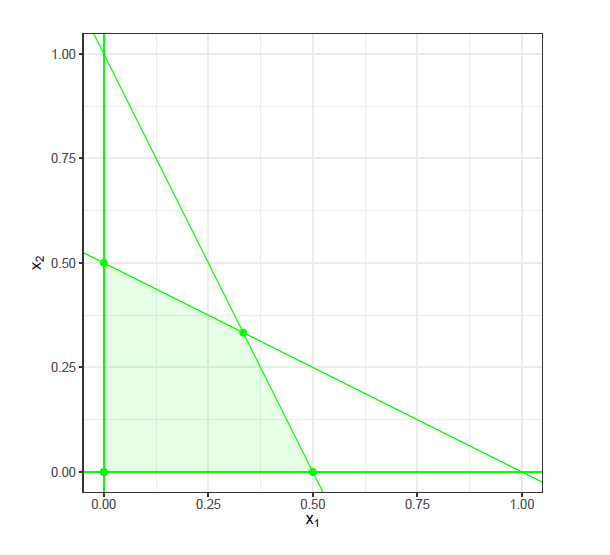
\includegraphics[width = 0.3\textwidth]{figure_man/linear-pro-example.png}
\end{center}

%<<echo = F>>=
%# plot polytope
%plotPoly = function(A, b) {

%  p = ggplot(data = data.frame(x = 0), mapping = aes(x = x))
%  p = p + geom_point(x = 0, y = 0, size = 2, color = "green")

%  for (i in 1:dim(A)[1]) {
%    p = p + geom_abline(intercept = b[i] / A[i, 2], slope = - A[i, 1] / A[i, 2], color = "green")
%  }

%  p = p + geom_segment(aes(x = 0, y = -Inf, xend = 0, yend = Inf), color = "green")
%  p = p + geom_segment(aes(x = -Inf, y = 0, xend = Inf, yend = 0), color = "green")

%  combs = combn(1:dim(A)[1], 2)

%  V = matrix(0, 0, 2)

%  for (i in 1:dim(combs)[2]) {

%    ind = combs[, i]

%    if (det(A[ind, ]) != 0) {
%      sol = solve(A[ind, ], b[ind])

%      if (all(A %*% sol <= b)) {
%        V = rbind(V, solve(A[ind, ], b[ind]))
%        p = p + geom_point(x = sol[1], y = sol[2], color = "green", size = 2)
%      }
%    }
%  }

%  V = as.data.frame(V)

%  center = apply(V, 2, mean)
%  Vdiff = V - center

%  ordering = vector(length = 0)

%  for (i in 1:dim(Vdiff)[1]) {
%    ordering = cbind(ordering, atan2(Vdiff[i, 1], Vdiff[i, 2]))
%  }

%  V = V[order(ordering), ]

%  p = p + geom_polygon(data = V, aes(x = V1, y = V2), fill = "green", alpha = 0.1)

%  p = p + coord_equal() + xlab(expression(x[1])) + ylab(expression(x[2]))


%  p = p + xlim(c(0, 1)) + ylim(c(0, 1)) + theme_bw()

%  p
%}
%@

%\vspace*{-0.5cm}

%<<echo = F, out.width = '50%', fig.align='center', warning = F>>=
%A = matrix(c(1, 2, -1, 0, 2, 1, 0, -1), ncol = 2)
%b = c(1, 1, 0, 0)

%plotPoly(A, b)
%@


\begin{itemize}
\item \textbf{(Sparse) Quantile regression}:

\begin{eqnarray*}
\min_{\bm{\beta}\in \R^p} && \frac{1}{n}\sum_{i = 1}^n \rho_\tau \left(y^{(i)} - \beta_0 -  \bm{\beta}^T\xv^{(i)}\right) \\
\text{s.t. } && \|\bm{\beta}\|_1 \le t
\end{eqnarray*}
where scalar $\beta_0$ and $\bm{\beta} \in \R^p$ are the quantile regression coefficients for $\tau \in [0,1]$, and $\rho_\tau(\cdot)$ is the check function defined as

\begin{footnotesize}
  $$
  \rho_\tau(s) = \begin{cases} \tau \cdot s & \text{for } s>0 \\ -1(1-\tau)\cdot s & \text{for } s\le0
  \end{cases}
  $$
\end{footnotesize}

When parameter $\tau = 1/2$, quantile regression amounts to median regression, least absolute error (LAE), or least absolute deviation (LAD). As in Lasso, $t\ge0$ is a tuning parameter. 

\item \textbf{Dantzig selector}:

\begin{eqnarray*}
\min_{\bm{\beta}\in \R^p} && \|\bm{\beta}\|_1 \\
\text{s.t. } && \| \bm{X}^T (\bm{X} \bm{\beta} - \bm{y})\|_\infty \le \lambda \,
\end{eqnarray*}
\end{itemize}

where $\bm{y} \in \R^n$, $\bm{X} \in \R^{n \times p}$, and $\lambda > 0$ is a tuning parameter. The infinity norm is defined as $\| x \|_\infty = \max\{|x_1|, \dots, |x_i|, \ldots, |x_n|\}$ is  

\lz

The Dantzig selector is similar (and behaves similar) to the Lasso and was introduced for variable selection in the seminal paper by Terence Tao and Emmanuel Cand\`es (see moodle page for reference).

\lz

Details about LPs in statistical estimation can be found, e.g., in the PhD thesis of \href{ttps://etd.ohiolink.edu/apexprod/rws_etd/send_file/send?accession=osu1222035715&disposition=inline}{\beamergotobutton{Yonggong Gao}}). 

\framebreak

W.l.o.g. Linear programming is specified using the so-called \textbf{standard form}.

\vspace*{-0.5cm}

\begin{eqnarray*}
\max_{\bm{x} \in \R^n} && \bm{c}^T\bm{x}\\
\text{s.t. } && \bm{A}\bm{x} \le \bm{b} \\
&& \bm{x} \ge 0
\end{eqnarray*}

The inequality constraints $\bm{Ax} \le \bm{b}$ ($\bm{A} \in \R^{m\times n}$, $\bm{b} \in \R^m$) and $\bm{x} \ge 0$ are to be understood componentwise.

\lz

The condition $\bm{x} \ge 0$ is known as the \textbf{non-negativity constraint} and the vector $\bm{c}$ is known as the \textbf{cost vector}.

%
% \begin{eqnarray*}
% &&\min_{\bm{x} \in \R^n} f(\bm{x})\\
% \text{u. d. N. } && g_i(\bm{x}) \le 0, h_j(\bm{x}) = 0,
% \end{eqnarray*}
%
% wobei $f: \R^n \to \R$, $g_i: \R^n \to \R$, $h_j: \R^n \to \R$ lineare Funktionen sind.

\framebreak

Linear optimization problems can be converted to the standard form by the following operations:

\begin{itemize}
\item Maximization instead of minimization: multiplication of the cost vector $\bm{c}$ by $-1$
\item Less than or equal instead of greater than or equal: multiply the inequality by $-1$
\item Equality instead of inequality: replace $\bm{a}_i\bm{x}=b_i$ with two conditions of inequality $\bm{a}_i\bm{x}\ge b_i$ and $\bm{a}_i\bm{x}\le b_i$
\item Variable without non-negativity constraint: replace $x_i$ with $x_i^+ - x_i^-$ with $x_i^+, x_i^- \ge 0$ (positive or negative part).
\end{itemize}

In the following we assume that the LP is given in standard form.

\framebreak

\textbf{Example:}

\lz

The example above

\vspace*{-1cm}
\begin{eqnarray*}
\min && - x_1 - x_2 \\
\text{s.t. } && x_1 + 2x_2 \le 1\\
&& 2x_1 + x_2 \le 1 \\
&& x_1, x_2 \ge 0
\end{eqnarray*}

can also be formulated as

\vspace*{-0.2cm}

\begin{eqnarray*}
\max && (1, 1) \begin{pmatrix} x_1 \\ x_2 \end{pmatrix} \\
\text{s.t. } &&  \begin{pmatrix}  1 &  2 \\  2 &  1 \end{pmatrix} \bm{x} \le \begin{pmatrix}  1 \\  1
\end{pmatrix} \\
&& \bm{x} \ge 0
\end{eqnarray*}

\end{vbframe}


\begin{vbframe}{Geometric interpretation}

Linear programming can be interpreted geometrically.

\lz

\textbf{Feasible set:}
\begin{itemize}
\item Let $\bm{a}_i \bm{x} \ge b_i$ be the i-th line of the inequality conditions.
\item The points that satisfy the linear system $\bm{a}_i \bm{x} = b_i$ form a hyperplane in $n$-dimensional space.
\item The vector $\bm{a}_i$ is perpendicular to the plane and is called the \textbf{normal vector}.
\framebreak
\item The set of points $\{\bm{x}: \bm{a}_i \bm{x} \ge b_i\}$ consists of points on the side of the hyperplane into which the normal vector points (\textbf{half-space}).

\vspace{0.2cm}
\begin{center}
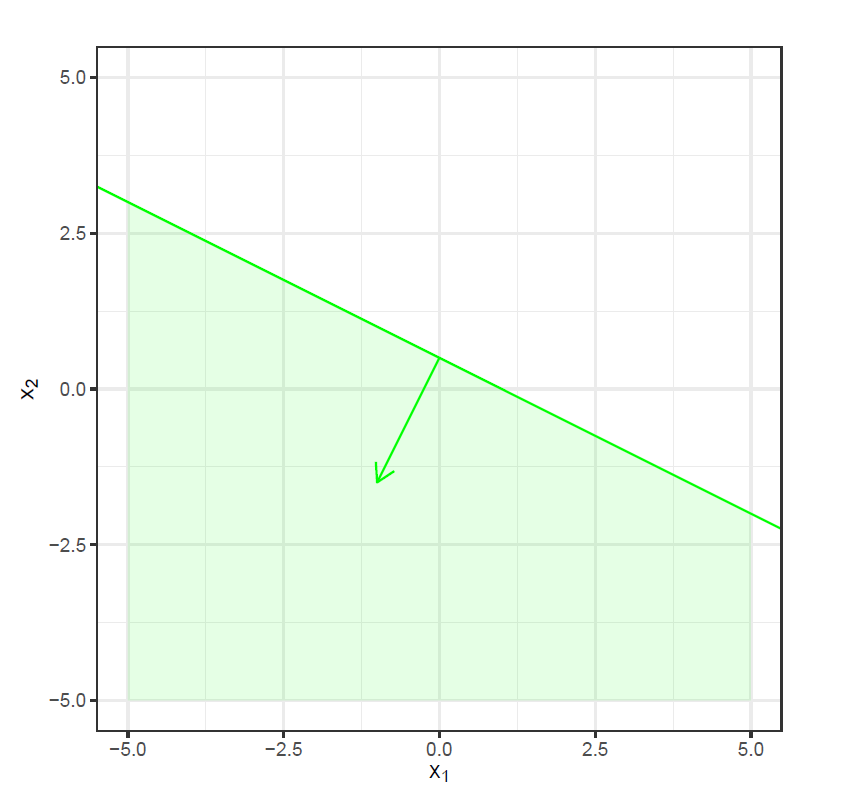
\includegraphics[width = 0.5\textwidth]{figure_man/geo-interpretation.png}
\end{center}


%<<fig.align='center', out.width='80%', echo = F, warning = F>>=
%f = function(x) b[1] / A[1, 2] - b[1] / A[1, 2] * x

%p = ggplot(data = data.frame(x = 0))
%p = p + geom_abline(slope = - b[1] / A[1, 2], intercept =  b[1] / A[1, 2], color = "green")
%p = p + geom_polygon(data = data.frame(x = c(-5, 5, 5, -5), y = c(-5, -5, f(5), f(-5))), aes(x = x, y = y), fill = "green", alpha = 0.1)
%p = p + geom_segment(aes(x = 0, y = f(0), xend = 0 - A[1, 1], yend = f(0) - A[1, 2]), arrow = arrow(length = unit(0.03, "npc")), color = "green")

%p = p + xlab(expression(x[1])) + ylab(expression(x[2]))

%p = p + theme_bw() + coord_equal()

%p = p + xlim(c(-5, 5))
%p = p + ylim(c(-5, 5))

%p
%@

\framebreak

\item Each of the $m$ inequalities divides the $n$-dimensional space into two halves.
\item \textbf{Claim:} The points that satisfy \textbf{all} inequalities form a \textbf{convex polytope}.
\end{itemize}

\begin{center}
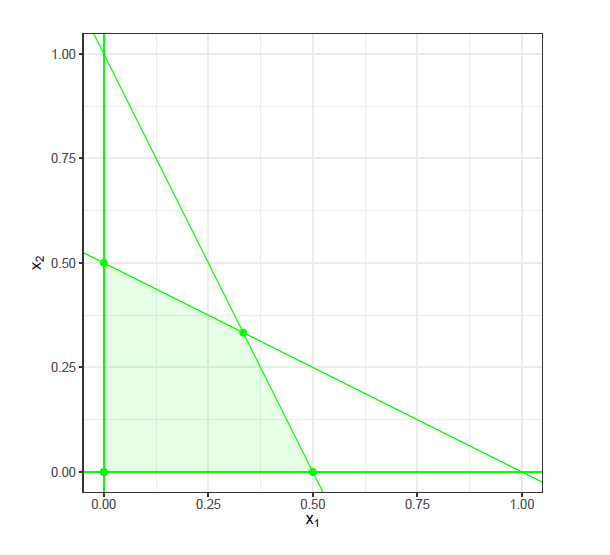
\includegraphics[width = 0.5\textwidth]{figure_man/linear-pro-example.png}
\end{center}


%<<echo = F, out.width = '60%', fig.align='center', warning = F>>=
%plotPoly(A, b)
%@


\framebreak

In geometry, a \textbf{polytope} denotes a generalized polygon in an arbitrary dimension. A polytope consists of several subpolytopes.

\begin{itemize}
\item A $0$ polytope is a single point,
\item A $1$ polytope is a line,
\item A $2$ polytope is a polygon, ...
\end{itemize}

In general, a $d$ polytope is formed from several $(d-1)$ polytopes (so-called facets) which in turn can have a $(d-2)$ polytope in common. Thus a $3$ polytope (e.g. a cube) has several sides / facets, some of which have common edges, etc.

\framebreak

The points for which $\bm{a}_i \bm{x} = b_i$ applies lie on the \textbf{facet} of the polytope.


\lz

The polytope which is defined by the inequalities $\bm{Ax} \ge \bm{b}$ is convex. For two points $\bm{x}_1, \bm{x}_2$, which lie in the polytope, any point that results from the convex combination of the two points, is again inside the polytope:

\begin{eqnarray*}
\bm{A}(\bm{x}_1 + t(\bm{x}_2 - \bm{x}_1)) &=& \bm{A}\bm{x}_1 + t(\bm{A}\bm{x}_2 - \bm{A}\bm{x}_1) \\ &=& (1 -t)\underbrace{\bm{A}\bm{x}_1}_{\ge \bm{b}} + t\underbrace{\bm{A}\bm{x}_2}_{\ge \bm{b}} \\ &\ge& (1 - t) \bm{b} + t \bm{b} = \bm{b} \qquad \text{for }t \in [0, 1])
\end{eqnarray*}

A polytope formed by the convex hull of $(n + 1)$ affin independent points in $\R^n$ is also called $n$-\textbf{simplex}.

\framebreak

\textbf{Objective function:}
\begin{itemize}
\item For the objective function, we consider the \textbf{contour lines}. Points that lie on the same contour line have the same objective function value.
\item In the linear case, the contours $y = \bm{c}^T \bm{x}$ are also a hyperplane for fixed $y$.
\item The vector $\bm{c}$ is again perpendicular to the respective contour lines.
\item The vector $\bm{c}$ can also be interpreted as a gradient. The \textbf{negative} gradient $- \bm{c}$ points in the direction of the \enquote{steepest} descent.
\framebreak
\item The value of the function becomes smaller when we go in the direction of the \textbf{negative gradient} $- \bm{c}$.

\begin{center}
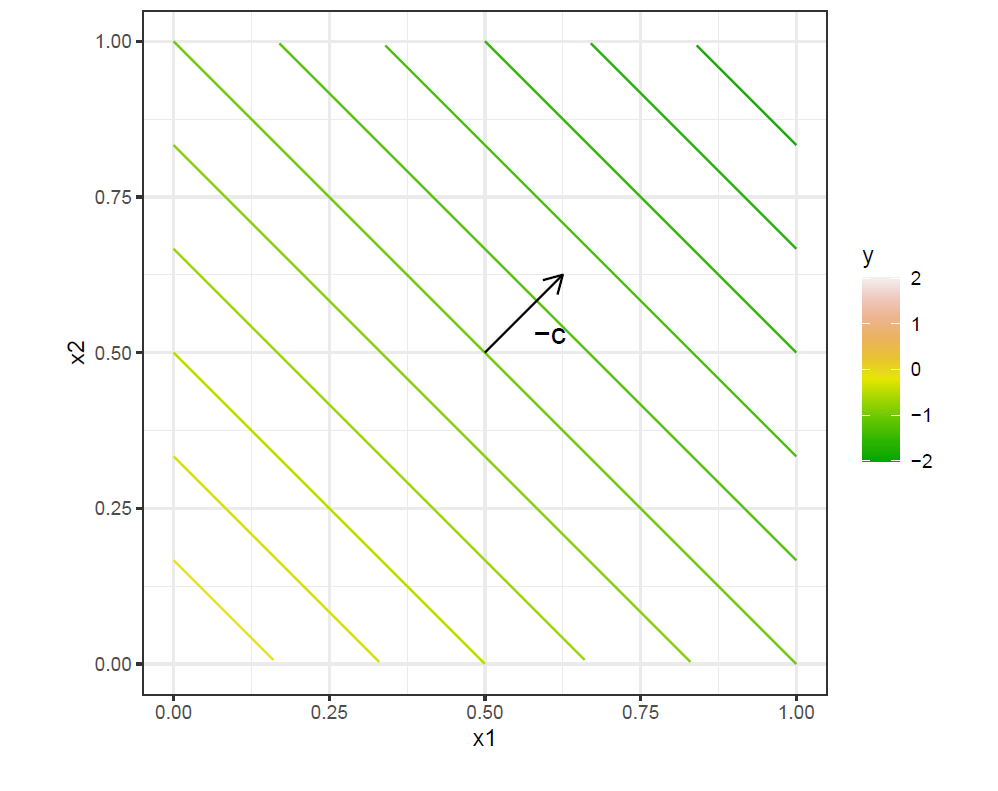
\includegraphics[width = 0.5\textwidth]{figure_man/negative-gradient.png}
\end{center}


%<<echo = F, out.width = '80%', fig.align='center', warning = F>>=
%f =  function(x, z) - z - x
%dd = expand.grid(x = seq(-2, 2, by = 0.01), z = seq(-2, 2, by = 1 / 6))
%dd %>% rowwise %>% mutate(y = f(x = x, z = z)) -> dd2

%p = ggplot() + geom_path(data = dd2, aes(x, y, col = z, group = z))
%p = p + scale_colour_gradientn(colours = terrain.colors(10))
%p = p + theme_bw() + xlim(c(0, 1)) + ylim(c(0, 1))
%p = p + xlab("x1") + ylab("x2") + labs(colour = "y")
%p = p + geom_segment(aes(x = 0.5, y = 0.5, xend = 0.625, yend = 0.625), arrow = arrow(length = unit(0.03, "npc")))
%p = p + geom_text(aes(x = 0.5, y = 0.5, label = "-c"), hjust = -1.5, vjust = -0.4, size = 5)

%p = p + coord_equal()

%p
%@

\framebreak
\item So we move the objective function \textbf{in the opposite direction} of the normal vector until the line just touches the polygon.

\begin{center}
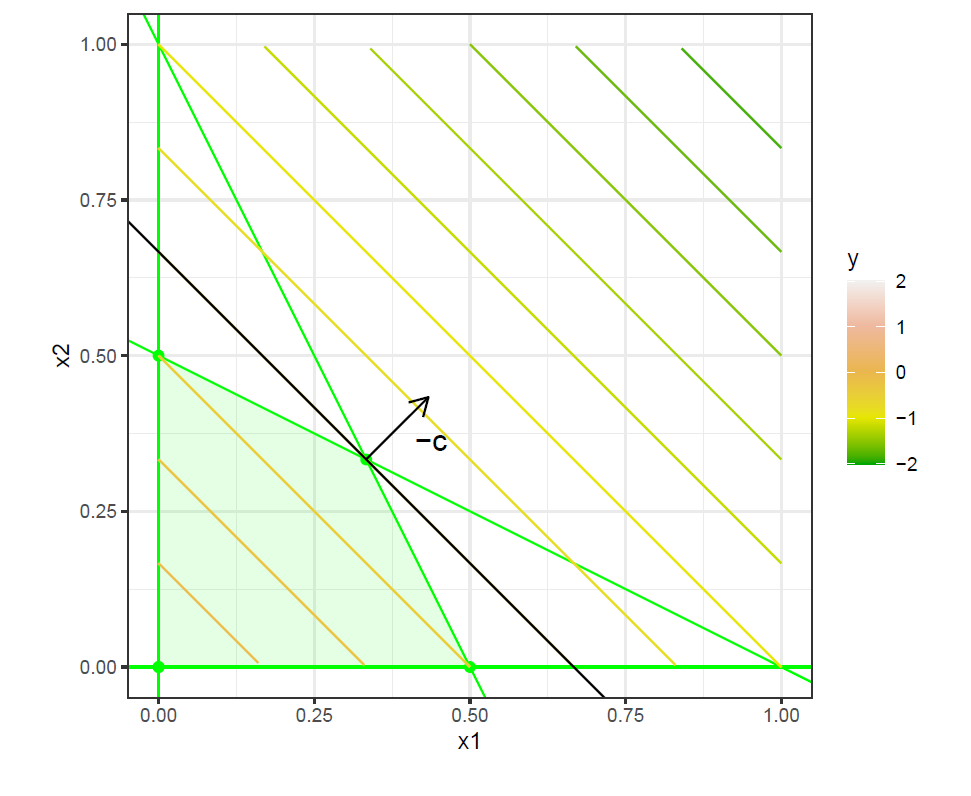
\includegraphics[width = 0.5\textwidth]{figure_man/opposite-direction.png}
\end{center}

%<<echo = F, out.width = '80%', fig.align='center', warning = FALSE, message = FALSE>>=
%p = plotPoly(A, b)

%p = p + geom_path(data = dd2, aes(x, y, col = z, group = z))

%p = p + scale_colour_gradientn(colours = terrain.colors(5))
%p = p + xlab("x1") + ylab("x2") + labs(colour = "y") + theme_bw()

%p = p + geom_abline(intercept = 2 / 3, slope = - 1, color = "black")
%p = p + geom_segment(aes(x = 1 / 3, y = 1 / 3, xend = 1 / 3 + 0.1, yend = 1 / 3 + 0.1), arrow = arrow(length = unit(0.03, "npc")))
%p = p + geom_text(aes(x = 1 / 3, y = 1 / 3, label = "-c"), hjust = -1.5, vjust = -0.4, size = 5)

%p = p + coord_equal()

%p
%@

\end{itemize}

\end{vbframe}

\begin{vbframe}{Solutions to LP}

There are three ways to solve Linear programming:

\begin{enumerate}
\item LP is \textbf{infeasible}, the feasible set is empty ($\mathcal{S} = \emptyset$)
\item LP is unconstrained
\item LP has at least one optimal solution
\end{enumerate}


\begin{center}
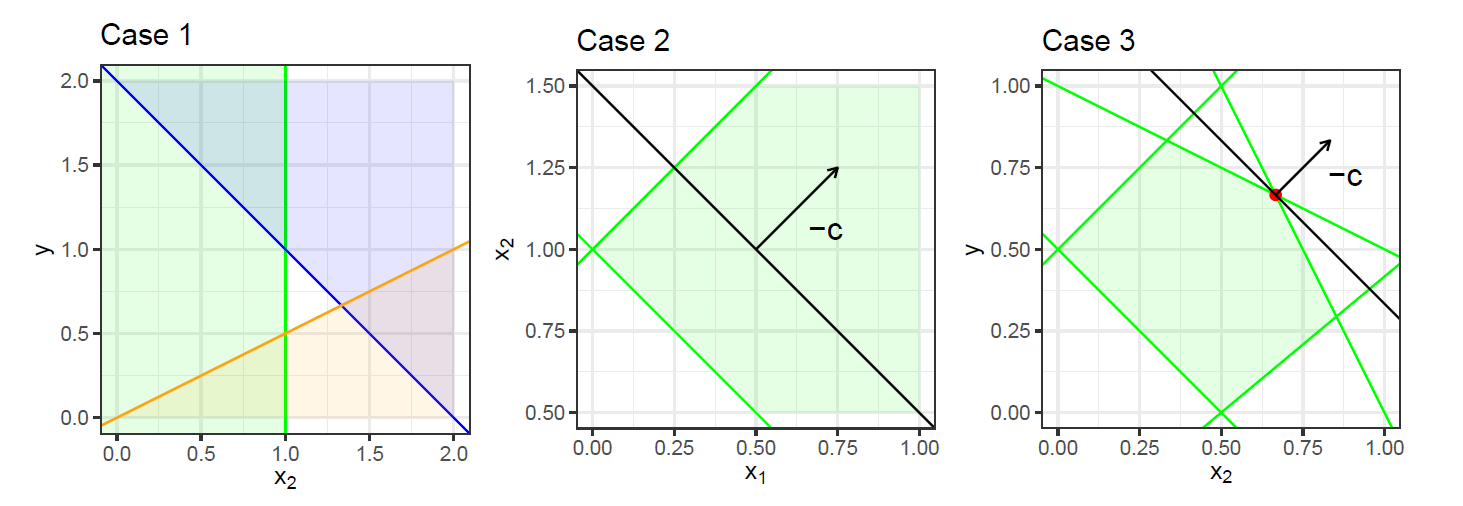
\includegraphics[width = 0.8\textwidth]{figure_man/solutions-lp.png}
\end{center}


\framebreak

\begin{itemize}
\item If LP is solvable and constrained (neither case 1 nor case 2), there is always an optimal point that can  \textbf{not} be convexly combined from other points in the polytope.
\item The optimal solution is then a corner, edge or side of the polytope.
\end{itemize}


\end{vbframe}

% \section{Algorithms for LP}

% \begin{vbframe}{Simplex algorithm}

% The Simplex algorithm is the most important method for solving Linear programming. It was published in 1947 by Georg Dantzig.

% \lz

% \textbf{Basic idea:} start from an arbitrary corner of the polytope. Run along this edge as long as the solution improves. Find a new edge, ...

% \lz

% \textbf{Output:} a path along the corners of the polytope that ends at the optimal point of the polytope.

% \lz

% Since linear programming is a \textbf{convex} optimization problem, the optimal corner found in this way is also a global optimum.

% \framebreak

% \begin{center}
% 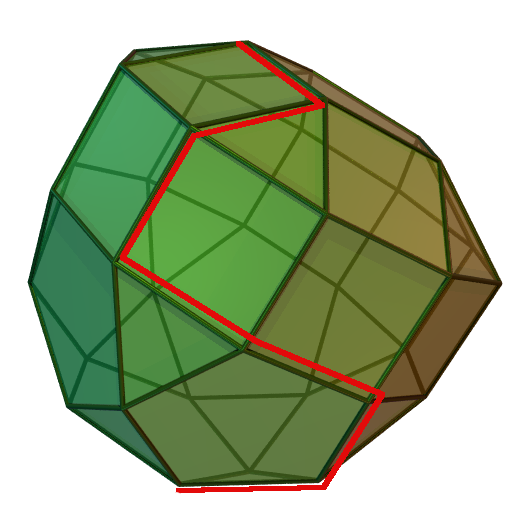
\includegraphics[width = 0.6\textwidth]{figure_man/simplex.png}
% \end{center}

% \framebreak

% The simplex algorithm can be divided into two steps:

% \begin{itemize}
% \item \textbf{Phase I:} determination of a \textbf{starting point}
% \item \textbf{Phase II:} determination of the \textbf{optimal solution}
% \end{itemize}

% To be able to start, a starting point must first be found in \textbf{Phase I}, i.e. a feasible corner $\bm{x}_0$.

% \lz

% In \textbf{phase II} this solution is iteratively improved by searching for an edge that improves the solution and running along it to the next corner.

% \framebreak

% \textbf{Phase I}:

% One way to find a starting point $\bm{x}_0$ is to solve a auxiliary linear problem with artificial variables $\bm{\epsilon}$:

% \begin{eqnarray*}
% \min_{\epsilon_1, ..., \epsilon_m} && \sum_{i = 1}^m \epsilon_i \\
% \text{s.t. } && \bm{Ax} + \bm{\epsilon} \ge \bm{b} \\
% && \epsilon_1, ..., \epsilon_m \ge 0\\
% && \bm{x} \ge 0
% \end{eqnarray*}

% \begin{itemize}
% \item A feasible starting point for the auxiliary problem is $\bm{x} = \bm{0}$ and $\epsilon_i = \begin{cases} 0 & \text{if } b_i < 0 \\
% b_i & \text{if } b_i \ge 0
% \end{cases}$
% \item We then apply phase II of the simplex algorithm to the auxiliary problem.
% \item If the original problem has a feasible solution, then the optimal solution of the auxiliary problem \textbf{must} be $\bm{\epsilon} = (0, ..., 0)$ (all artificial variables disappear) and the objective function is $0$.
% \item If we find a solution with $\bm{\epsilon} = \bm{0}$, then we have found a valid starting point.
% \item If we do not find a solution with $\bm{\epsilon} = \bm{0}$, the problem can not be solved.
% \end{itemize}

% \framebreak

% \textbf{Example:}

% \begin{eqnarray*}
% \min_{\bm{x} \in \R^2} && -x_1 - x_2 \\
% \text{s.t. } && x_1 - x_2 \ge - 0.5 \\
% && - x_1 - 2 x_2 \ge - 2 \\
% && - 2x_1 - x_2 \ge - 2 \\
% && - x_1 + x_2 \ge - 0.5 \\
% && \bm{x} \ge 0
% \end{eqnarray*}

% A starting point is the corner $\bm{(0, 0)}$.

% \framebreak

% \begin{center}
% 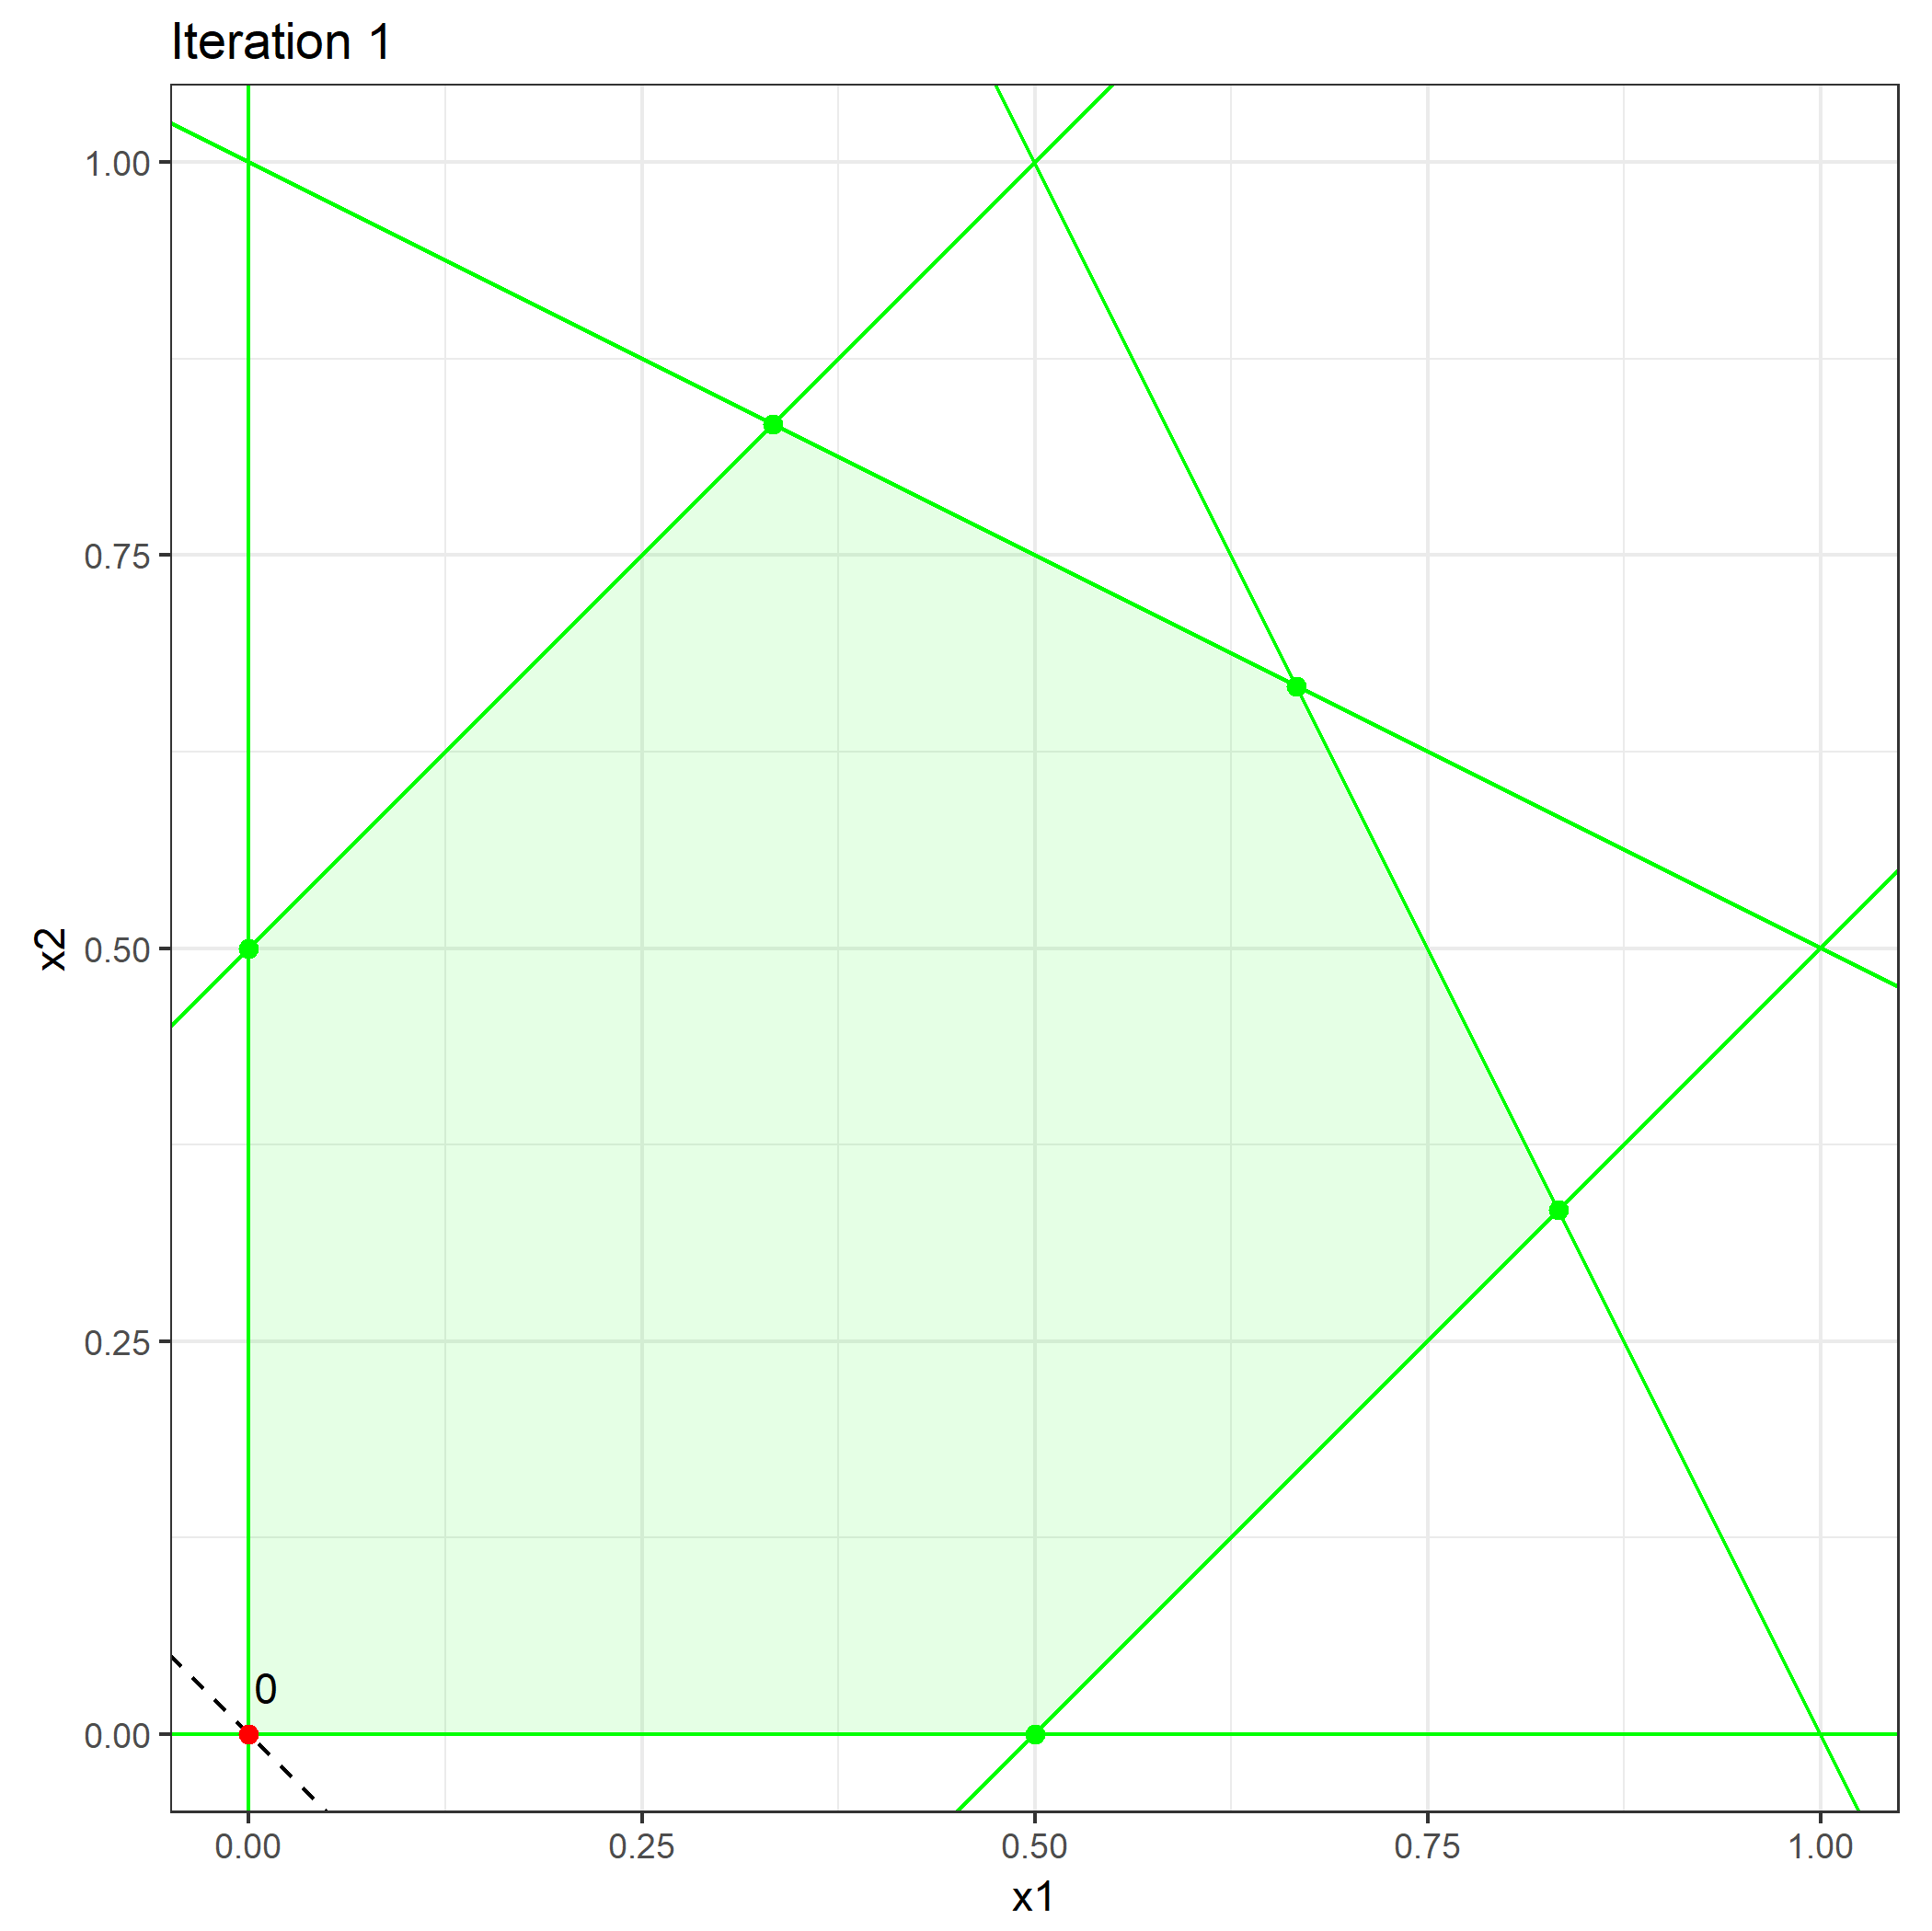
\includegraphics[width = 0.6\textwidth]{figure_man/simplex_implementation/iter1.png}
% \end{center}

% \framebreak

% \begin{center}
% 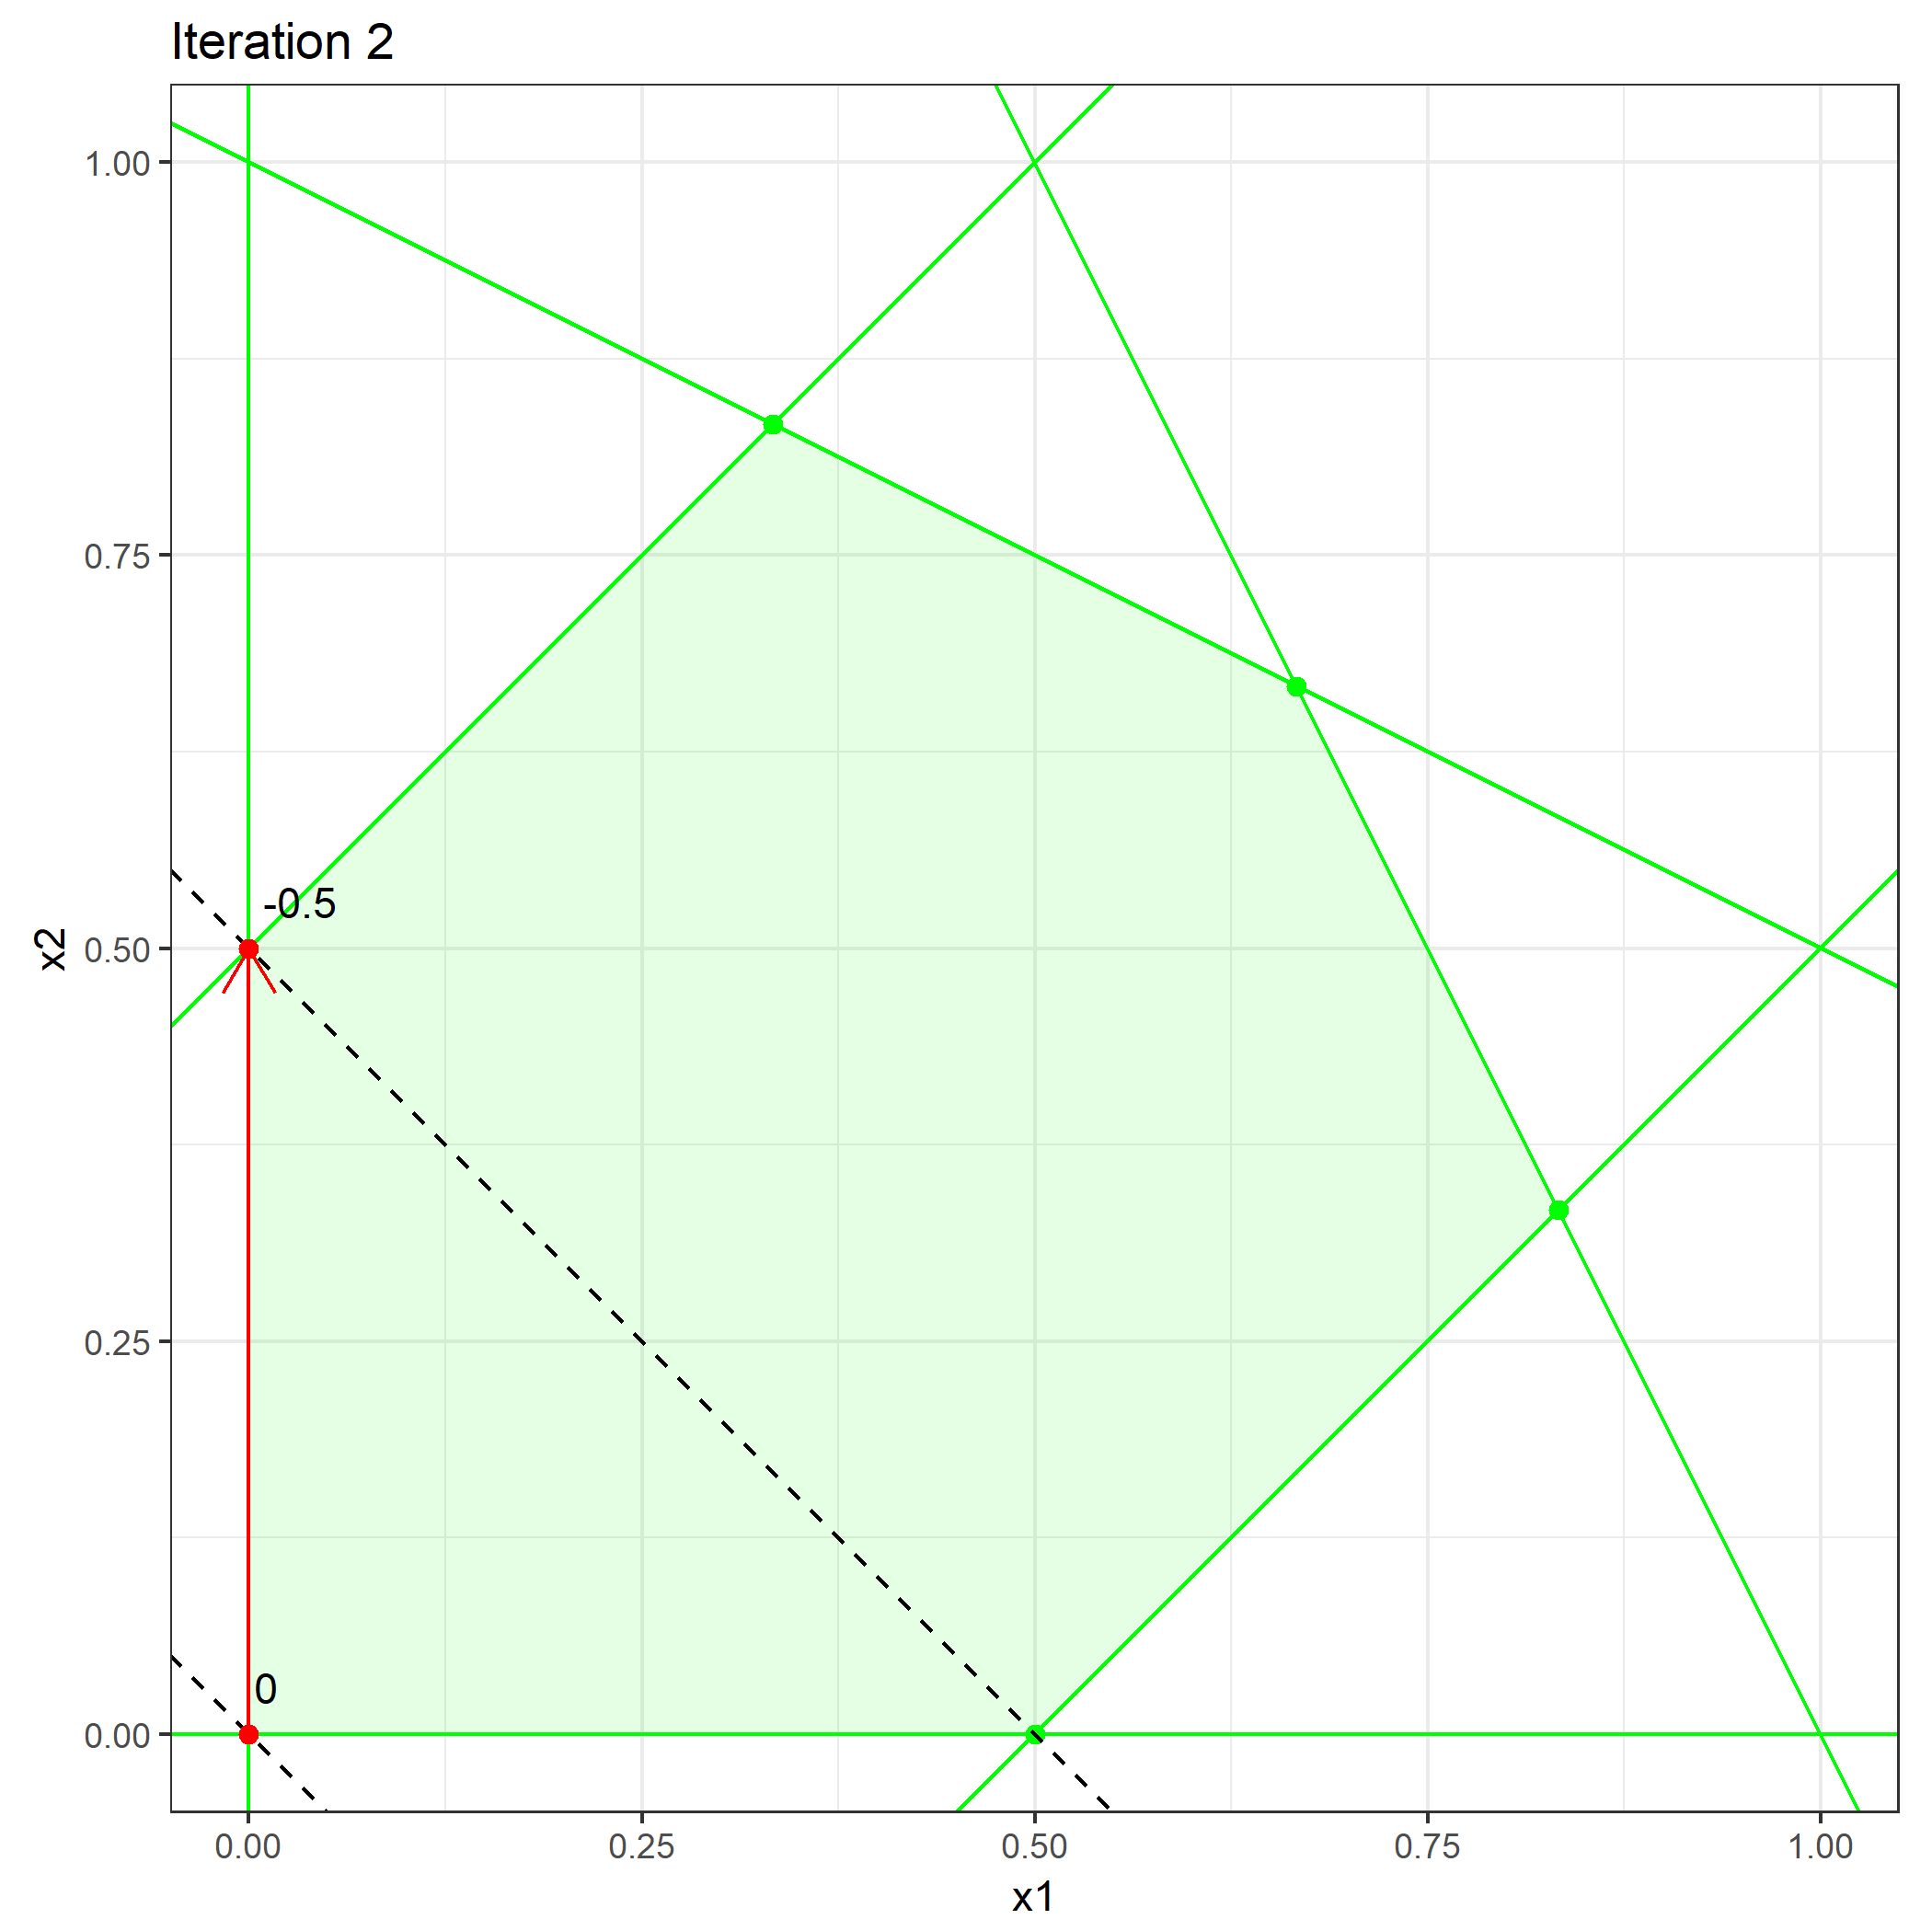
\includegraphics[width = 0.6\textwidth]{figure_man/simplex_implementation/iter2.png}
% \end{center}

% \framebreak

% \begin{center}
% 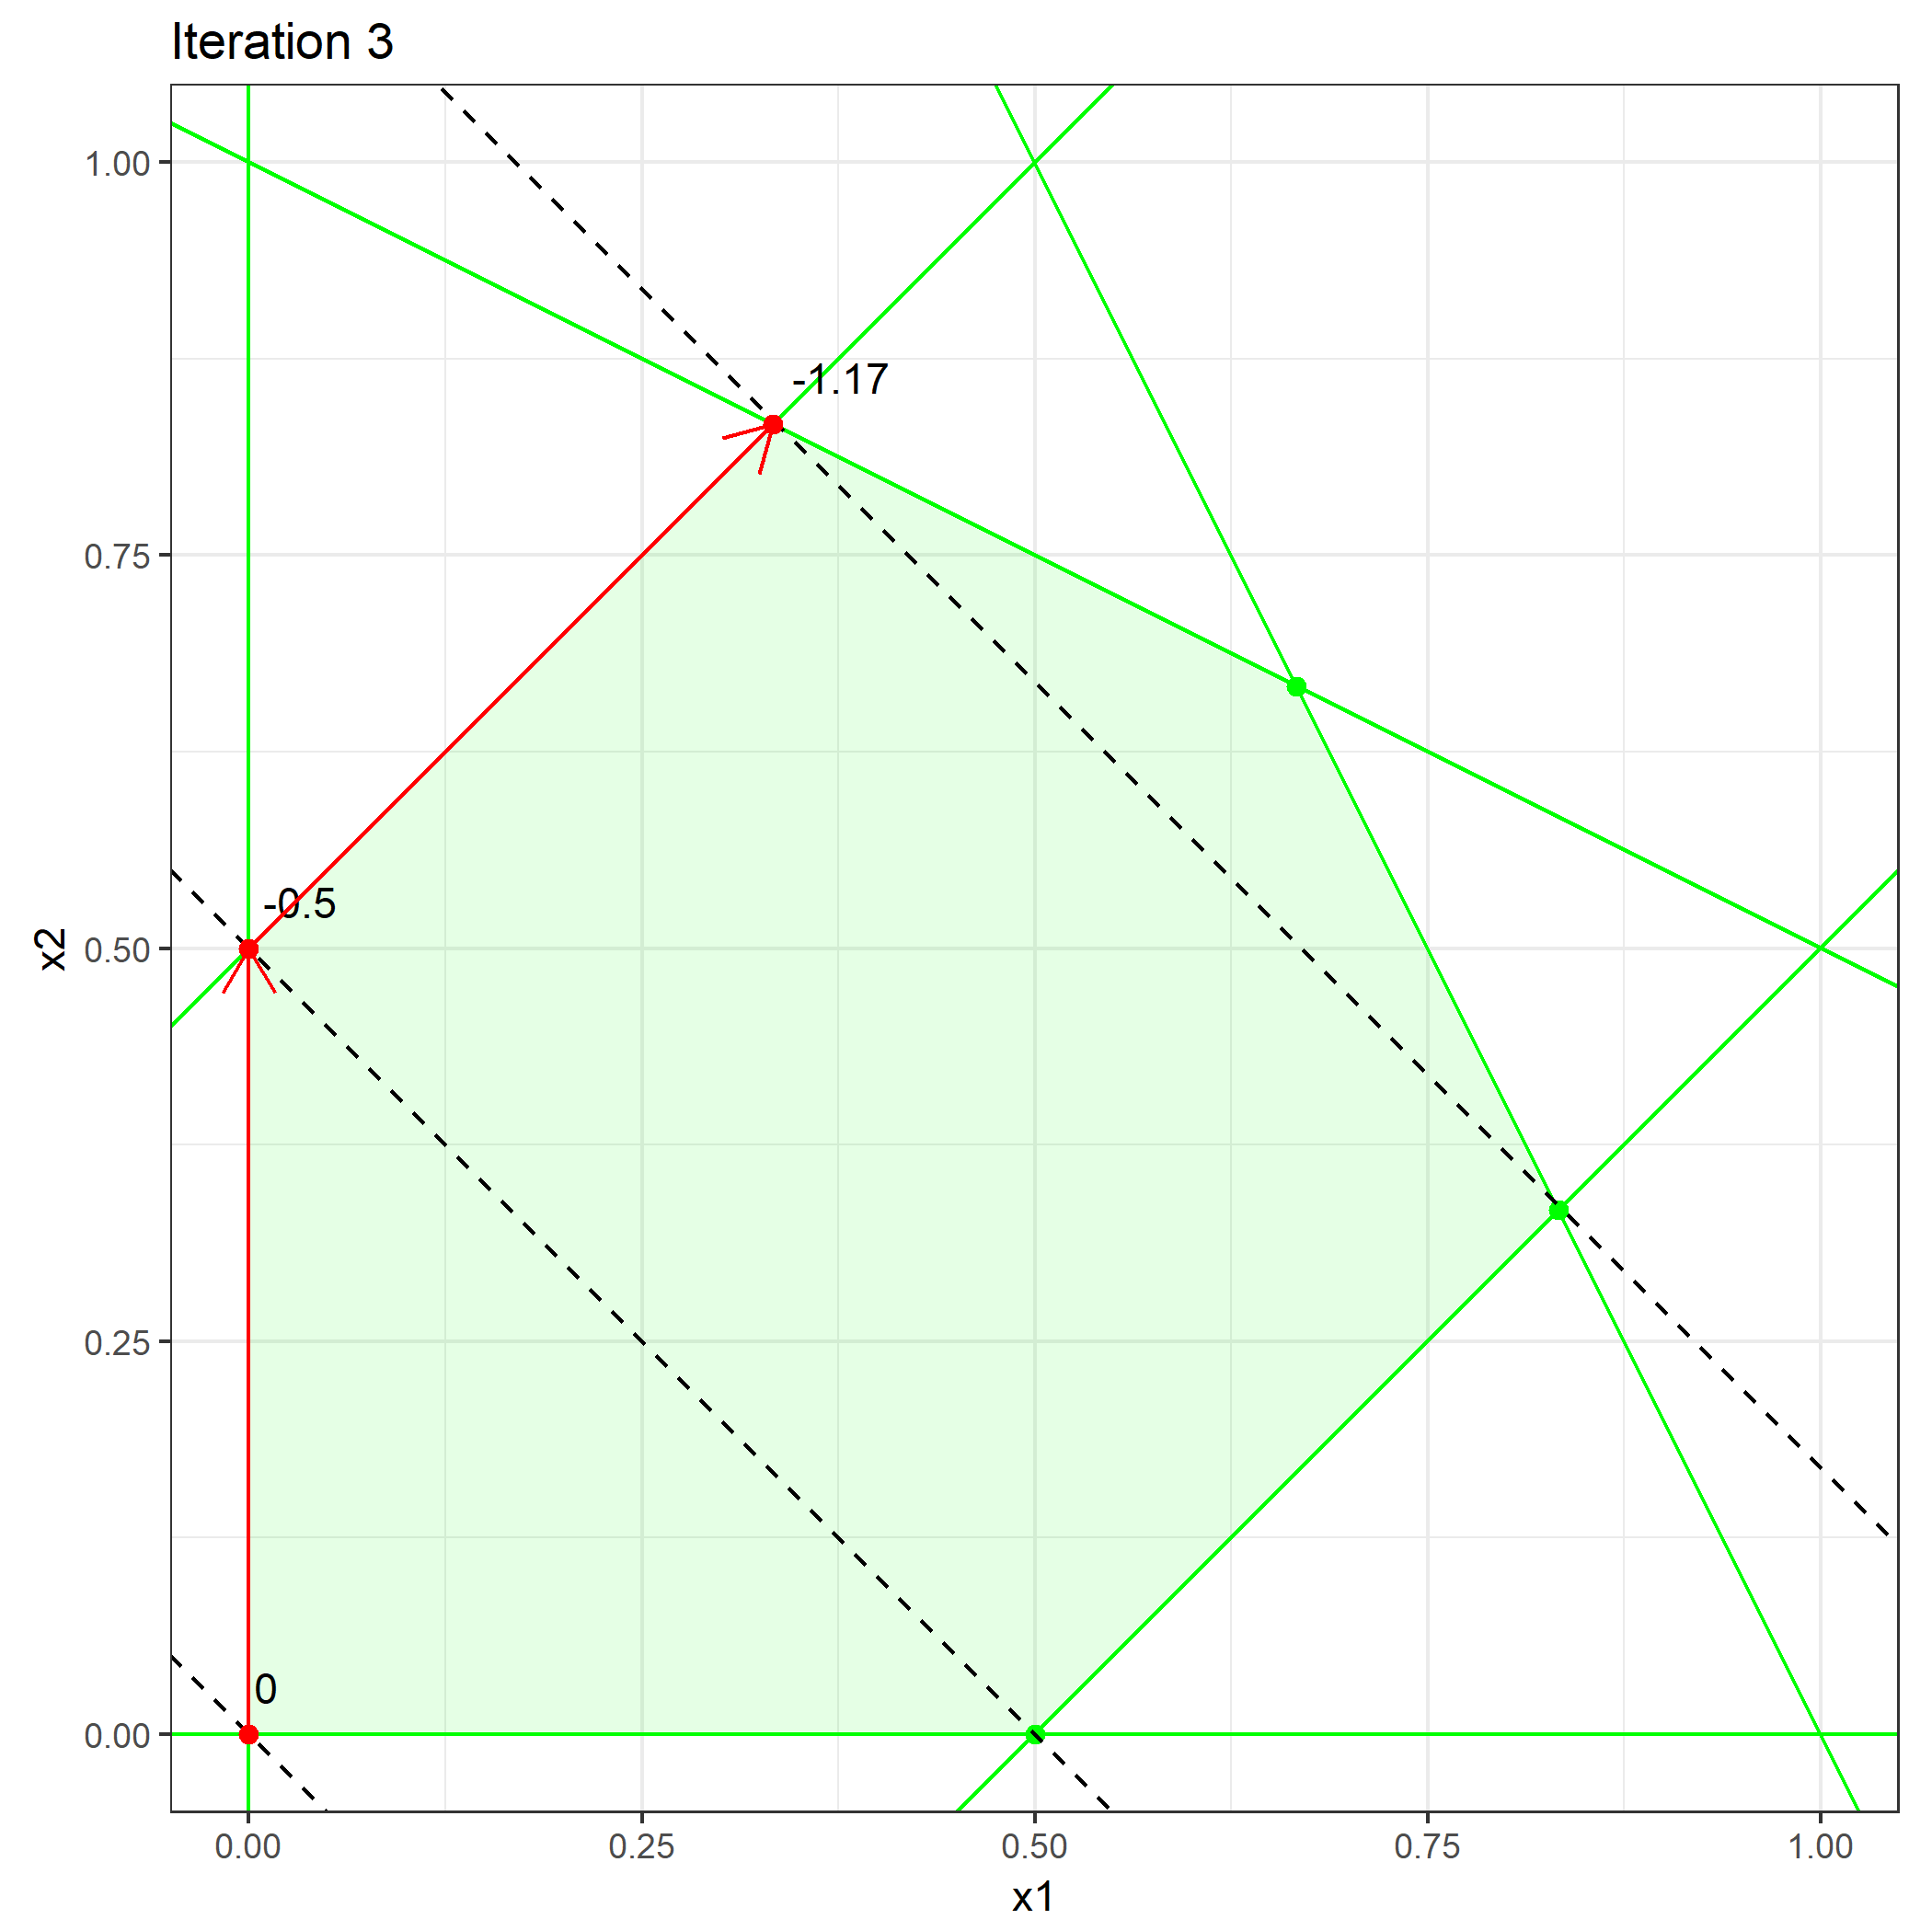
\includegraphics[width = 0.6\textwidth]{figure_man/simplex_implementation/iter3.png}
% \end{center}

% \framebreak

% \begin{center}
% 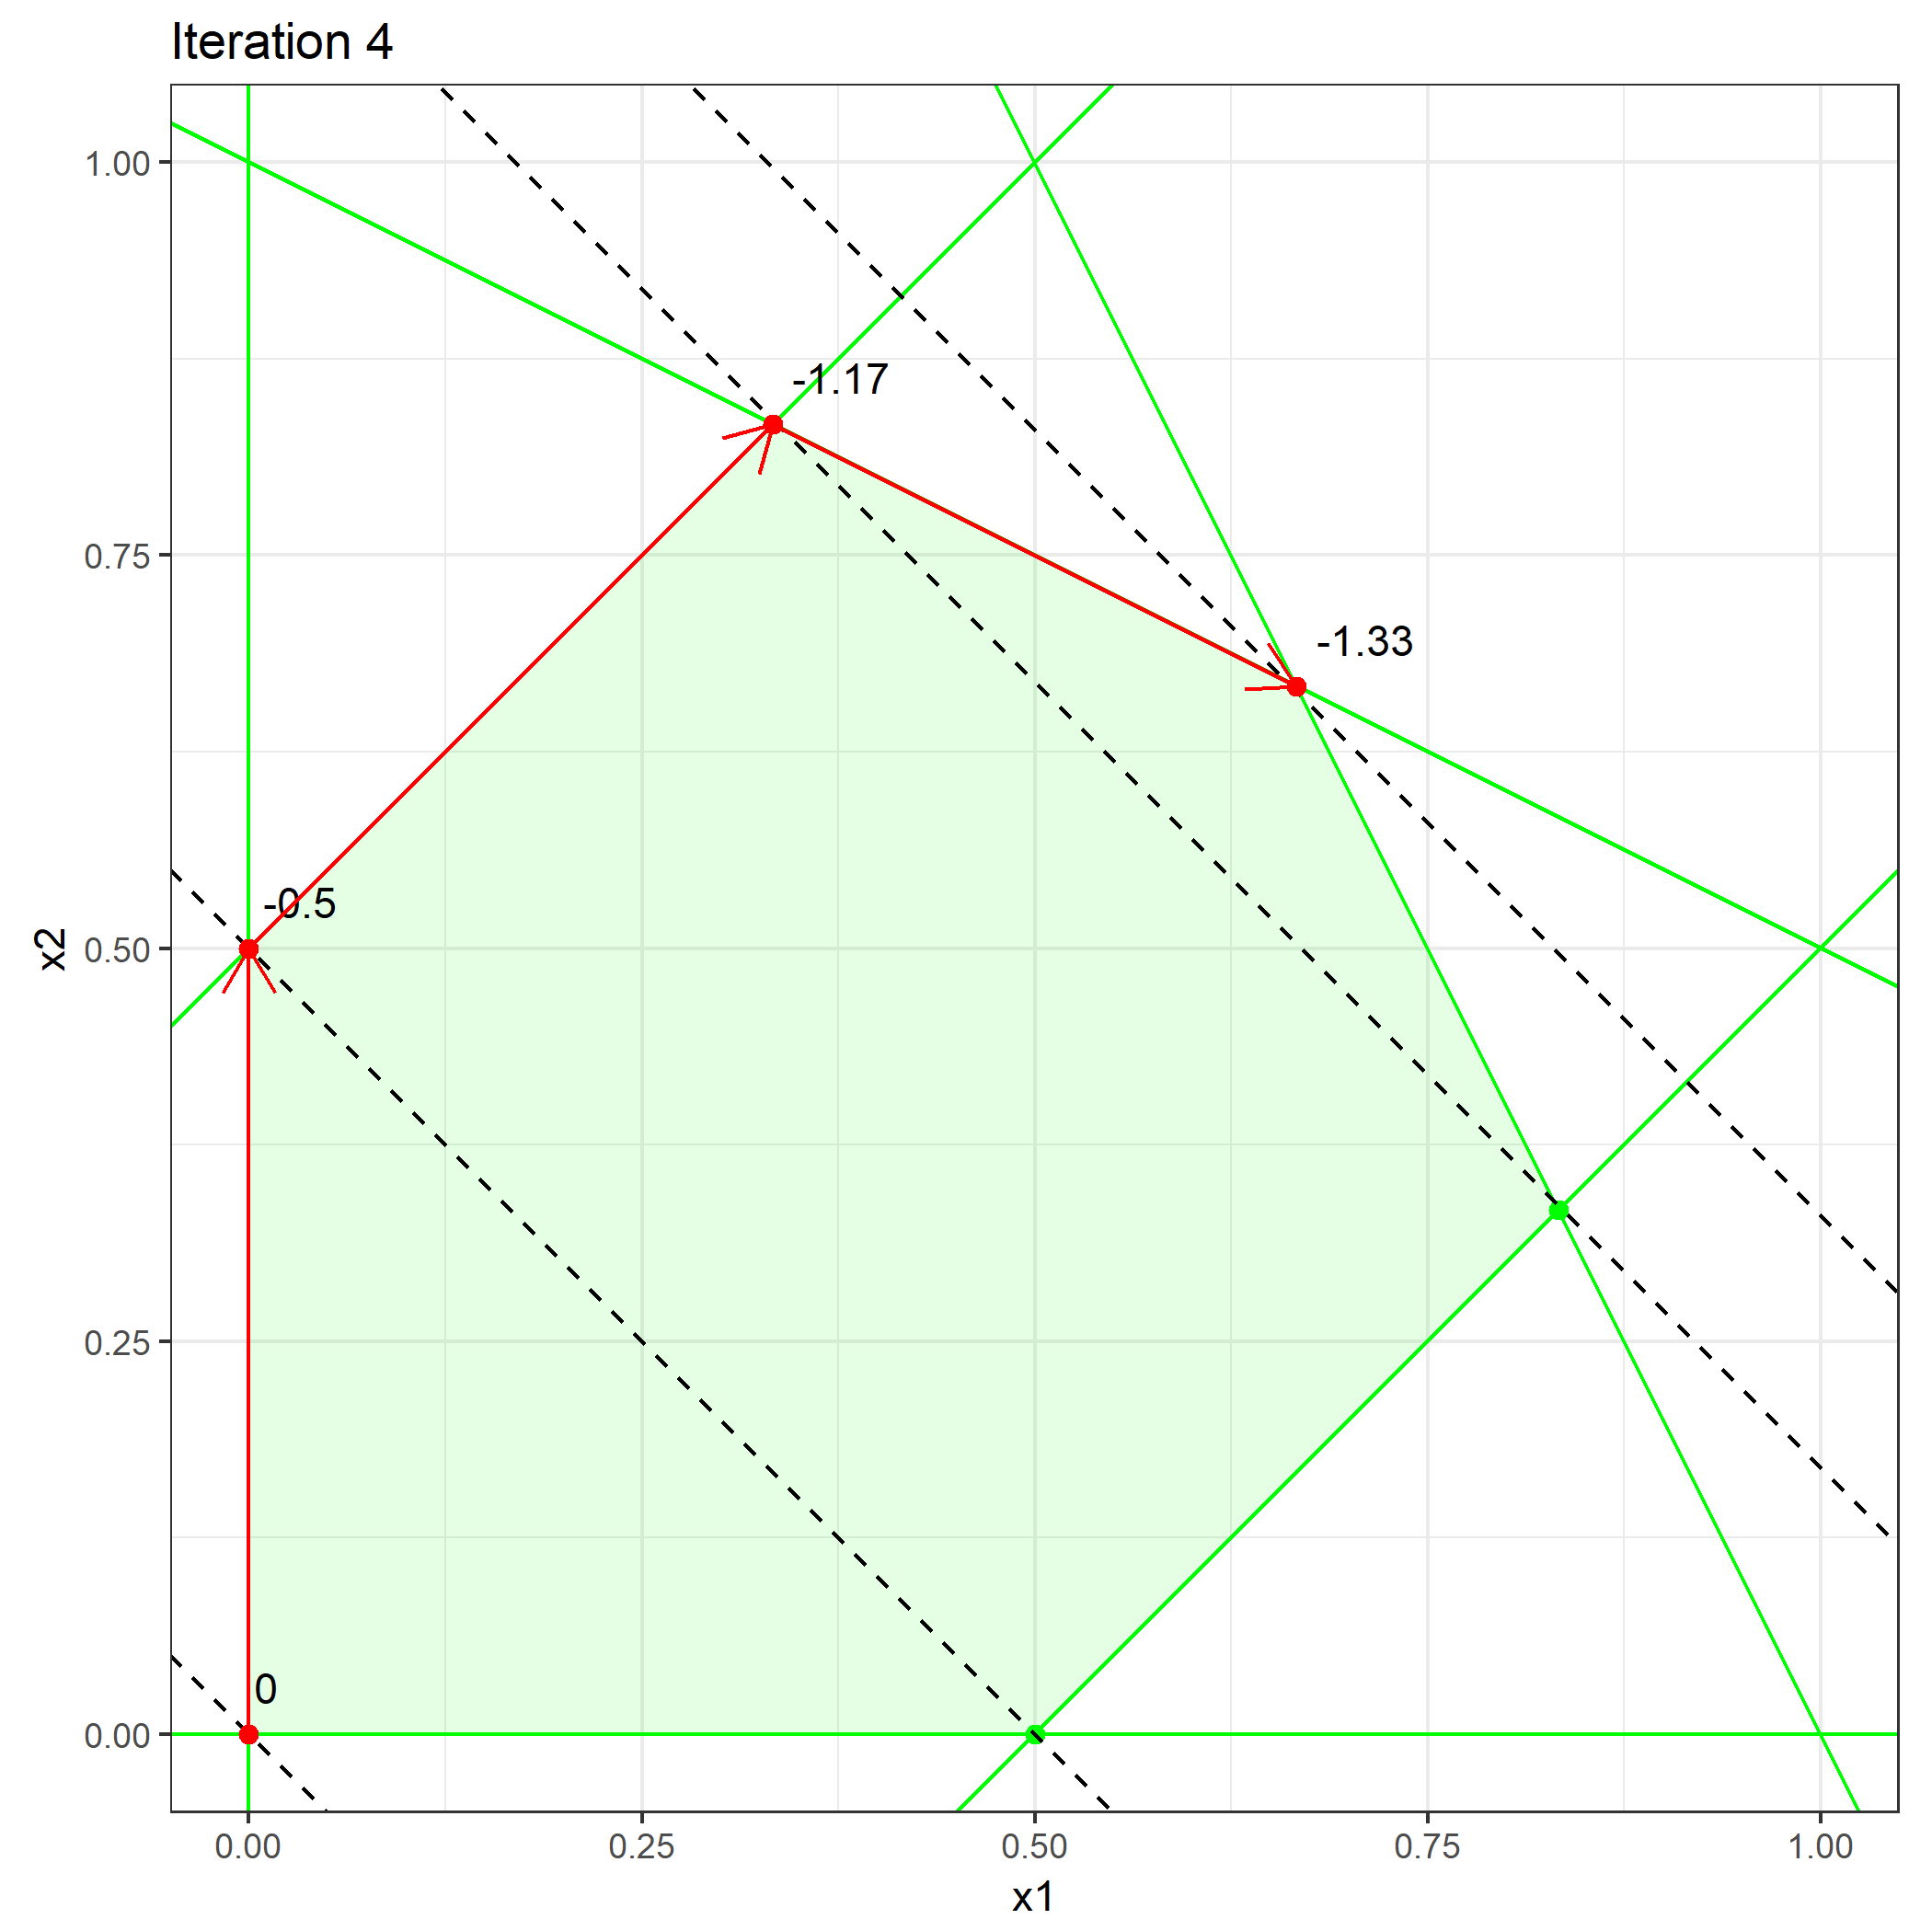
\includegraphics[width = 0.6\textwidth]{figure_man/simplex_implementation/iter4.png}
% \end{center}

% \end{vbframe}

% % \begin{vbframe}{Komplexität des Simplex Algorithmus}
% %
% % \end{vbframe}

% \section{Duality}

% \begin{vbframe}{Duality: introductory example}

% \textbf{Example:}

% A bakery sells brownies for $50$ ct and mini cheesecakes for $80$ ct each. The two products contain the following ingredients

% \begin{center}
% \begin{tabular}{ r c c c}
%     & \text{Chocolate} & \text{Sugar} & \text{Creamcheese} \\
%     \hline
%   \text{Brownie} & 3 & 2 & 2 \\
%   \text{Cheesecake} & 0 & 4 & 5
% \end{tabular}
% \end{center}

% A student wants to minimize his expenses, but at the same time eat at least $6$ units of chocolate, $10$ units of sugar and $8$ units of creamcheese.

% \framebreak

% He is therefore confronted with the following optimization problem:

% \begin{eqnarray*}
% \min_{\bm{x}\in \R^2} && 50x_1 + 80x_2 \\
% \text{s.t. } && 3x_1 \ge 6 \\
% && 2x_1 + 4x_2 \ge 10 \\
% && 2x_1 + 5x_2 \ge 8 \\
% && \bm{x} \ge 0
% \end{eqnarray*}

% \framebreak

% The solution of the Simplex algorithm:
% \vspace{0.3cm}

% \footnotesize
% \begin{verbbox}
% res = solveLP(cvec = c, bvec = b, Amat = A)
% summary(res)
% ##
% ##
% ## Results of Linear Programming / Linear Optimization
% ##
% ## Objective function (Minimum): 220
% ##
% ## Solution
% ## opt
% ## 1 2.0
% ## 2 1.5
% \end{verbbox}
% \col

% %<<echo = F>>=
% %A = - matrix(c(3, 2, 2, 0, 4, 5), ncol = 2)
% %b = - c(6, 10, 8)
% %c = c(50, 80)
% %@

% %<<>>=
% %res = solveLP(cvec = c, bvec = b, Amat = A)
% %summary(res)
% %@

% \framebreak
% \normalsize
% The baker informs the supplier that he needs at least $6$ units of chocolate, $10$ units of sugar and $8$ units of creamcheese to meet the student's requirements.

% \lz

% The supplier asks himself how he must set the prices for chocolate, sugar and creamcheese ($\alpha_1, \alpha_2, \alpha_3$) such that he can

% \begin{itemize}
% \item maximize his revenue
% $$
% \max_{\bm{\alpha} \in \R^3}6 \alpha_1 + 10 \alpha_2 + 8 \alpha_3
% $$
% \item and at the same time ensure that the baker buys from him (purchase cost $\le$ selling price)
% \begin{eqnarray*}
% 3\alpha_1 + 2\alpha_2 + 2\alpha_3 &\le& 50 \qquad \text{Brownie} \\
% 4\alpha_2 + 5\alpha_3 &\le& 80 \qquad \text{Cheesecake}
% \end{eqnarray*}

% \end{itemize}

% \framebreak

% The presented example is known as a \textbf{dual problem}. The variables $\alpha_i$ are called \textbf{dual variables}.

% \lz

% In an economic context, dual variables can often be interpreted as \textbf{shadow prices} for certain goods.

% \lz

% If we solve the dual problem, we see that the dual problem has the same objective function value as the primal problem. This is later referred to as \textbf{strong duality}.

% % \lz
% %
% % Der Lieferant sollte eine Einheit Schokolade für mindestens $\alpha_1$ verkaufen, der Bäcker aber höchstens zu $\alpha_1$ einkaufen.
% \framebreak
% \footnotesize
% \begin{verbbox}
% res = solveLP(cvec = c, bvec = b, Amat = A, maximum = T)
% summary(res)
% ##
% ##
% ## Results of Linear Programming / Linear Optimization
% ##
% ## Objective function (Maximum): 220
% ##
% ## Solution
% ## opt
% ## 1 3.333333
% ## 2 20.000000
% ## 3 0.000000
% \end{verbbox}
% \col

% %<<echo = F>>=
% %A = matrix(c(3, 0, 2, 4, 2, 5), ncol = 3)
% %b = c(50, 80)
% %c = c(6, 10, 8)
% %@

% %<<>>=
% %res = solveLP(cvec = c, bvec = b, Amat = A, maximum = T)
% %summary(res)
% %@


% % \textbf{Beispiel:} Eine Firma stellt Tische und Stühle her und verkauft diese für $30$ Euro (Tisch),  $20$ Euro (Stuhl). Hierfür gibt es $3$ Maschinen, die jeweils nur eine gewisse Zeit zur Verfügung stehen.
% %
% % \lz
% %
% % In der Tabelle ist aufgelistet, wie viel Stunden die jeweilige Maschine für Stuhl bzw. Tisch benötigt.
% %
% % \begin{center}
% % \begin{tabular}{ r | c c | c}
% %   \text{Maschine}  & \text{Stuhl} & \text{Tisch} & \text{Verfügbarkeit (in h)} \\
% %     \hline
% %   M_1 & 3 & 2 & 2 \\
% %   M_2 & 0 & 4 & 5 \\
% %   M_3 & 0 & 4 & 5
% %
% % \end{tabular}
% % \end{center}

% \end{vbframe}

% \normalsize
% \begin{vbframe}{Mathematical intuition}

% The example explained duality from an economic point of view. But what is the mathematical intuition behind duality?

% \lz

% \textbf{Idea: } In minimization problems one is often interested in \textbf{lower bounds} of the objective function. How could we derive a lower bound for the problem above?

% \lz

% If we \enquote{skilfully} multiply the three inequalities by factors and add factors (similar to a linear system), we can find a lower bound.

% \framebreak
% \vspace*{-1.6cm}

% \begin{eqnarray*}
% \min_{\bm{x}\in \R^2} && 50x_1 + 80x_2  \\
% \text{s.t. } && 3x_1 \ge 6 \quad \vert\textcolor{green}{\cdot 5}\\
% && 2x_1 + 4x_2 \ge 10 \quad \vert \textcolor{green}{\cdot 5} \\
% && 2x_1 + 5x_2 \ge 8 \quad \vert \textcolor{green}{\cdot 12} \\
% && \bm{x} \ge 0
% \end{eqnarray*}

% \vspace*{-0.2cm}

% If we add up the constraints we obtain

% \vspace*{-0.5cm}
% \begin{eqnarray*}
% & & \textcolor{green}{5} \cdot (3x_1) + \textcolor{green}{5} \cdot (2x_1 + 4x_2) + \textcolor{green}{12} \cdot (2x_1 + 5x_2)
% \\ &=& 15x_1 + 10x_1 + 24x_1 + 20x_2 + 60x_2 = 49 x_1 + 80 x_2 \\
% &\ge& 30 + 50 + 96 = 176
% \end{eqnarray*}

% Since $x_1 \ge 0$ we found a lower bound because

% $$
% 50x_1 + 80 x_2 \ge 49 x_1 + 80 x_2 \ge 176.
% $$

% \framebreak

% Maybe we could have transformed the equations more cleverly and then found a \textbf{better} lower bound. We replace the multipliers $5, 5, 12$ with $\alpha_1, \alpha_2, \alpha_3$ and demand (as a condition for a lower bound).

% % \begin{eqnarray*}
% % \min_{\bm{x}\in \R^2} && 50x_1 + 80x_2  \\
% % \text{u. d. N. } && 3x_1 \ge 6 \quad \vert \textcolor{green}{\cdot \alpha_1}\\
% % && 2x_1 + 4x_2 \ge 10 \quad \vert \textcolor{green}{\cdot \alpha_2} \\
% % && 2x_1 + 5x_2 \ge 8 \quad \vert \textcolor{green}{\cdot \alpha_3} \\
% % && \bm{x} \ge 0
% % \end{eqnarray*}
% %
% % \framebreak

% \vspace*{-0.5cm}

% \begin{eqnarray*}
% && 50x_1 + 80x_2 \ge \textcolor{green}{\alpha_1} (3x_1) + \textcolor{green}{\alpha_2} (2x_1 + 4x_2) + \textcolor{green}{\alpha_3} (2x_1 + 5x_2) \\ &=& (3 \textcolor{green}{\alpha_1} + 2  \textcolor{green}{\alpha_2} + 2 \textcolor{green}{\alpha_3}) x_1 + (4  \textcolor{green}{\alpha_2} + 5 \textcolor{green}{\alpha_3}) x_2
% \end{eqnarray*}

% or equivalently

% \vspace*{-0.5cm}
% \begin{eqnarray*}
% 3 \textcolor{green}{\alpha_1} + 2  \textcolor{green}{\alpha_2} + 2 \textcolor{green}{\alpha_3} \le 50, \\
% 4  \textcolor{green}{\alpha_2} + 5 \textcolor{green}{\alpha_3} \le 80.
% \end{eqnarray*}

% The lower bound (right-hand side of the inequality) is given by

% $$
% \textcolor{green}{\alpha_1} \cdot 6 + \textcolor{green}{\alpha_2} \cdot 10 + \textcolor{green}{\alpha_3} \cdot 8.
% $$

% \framebreak

% We are interested in a \textbf{largest possible} lower bound, because it gives us the most information. As an optimization problem

% \begin{eqnarray*}
% \max_{\bm{\alpha} \in \R^3} && 6 \alpha_1 + 10 \alpha_2 + 8 \alpha_3 \\
% \text{s.t. } && 3\alpha_1 + 2\alpha_2 + 2\alpha_3 \le 50 \\
% && 4\alpha_2 + 5\alpha_3 \le 80\\
% && \bm{\alpha} \ge 0.
% \end{eqnarray*}


% \end{vbframe}



% \begin{vbframe}{Duality}

% We denote

% \vspace*{-0.2cm}
% \begin{eqnarray*}
% \max_{\bm{\alpha} \in \R^m} && g(\bm{\alpha}) := \bm{\alpha}^T\bm{b}\\
% \text{s.t. } && \bm{\alpha}^T\bm{A} \le \bm{c}^T \\
% && \bm{\alpha} \ge 0
% \end{eqnarray*}

% as the \textbf{dual problem} of

% \begin{eqnarray*}
% \min_{\bm{x} \in \R^n} && f(\bm{x}) := \bm{c}^T\bm{x}\\
% \text{s.t. } && \bm{A}\bm{x} \ge \bm{b} \\
% && \bm{x} \ge 0
% \end{eqnarray*}

% (\textbf{primal problem}).

% \framebreak

% Duality overview:

% \begin{footnotesize}
% \begin{center}
%     \begin{tabular}{c | c | c | c}
%     & $\begin{array}{c} \text{Primal} \\ \text{(minimize)} \end{array}$ & $\begin{array}{c} \text{Dual} \\ \text{(maximize)} \end{array}$ \\
%     \hline
%     \multirow{3}{*}{$\begin{array}{c} \text{condition} \end{array}$} & $\le$ & $\le 0$ & \multirow{3}{*}{variable} \\
%   & $\ge$ & $\ge 0$ & \\
%     & $=$ & unconstrained & \\
%     \hline
%     \multirow{3}{*}{variable} & $\ge 0 $ & $\le$ & \multirow{3}{*}{$\begin{array}{c} \text{condition} \end{array}$}\\
%     & $\le 0$ &  $\ge$ & \\
%     & unconstrained & $=$ & \\
% \hline
%     \end{tabular}
% \end{center}
% \end{footnotesize}
% \end{vbframe}

% \begin{vbframe}{Duality theorem}

% In general, the \textbf{weak duality theorem}$^{(*)}$ applies to all feasible $\bm{x}, \bm{\alpha}$

% $$
% g(\bm{\alpha}) = \bm{\alpha}^T\bm{b} \le \bm{c}^T\bm{x}  = f(\bm{x})
% $$

% The value of the dual function is therefore \textbf{always} a lower bound for the objective function value of the primal problem.

% \lz

% \textbf{Proof:}
% $\bm{\alpha}^T\bm{b} \overset{\bm{Ax} \ge b}{\le}\bm{\alpha}^T\bm{Ax} \overset{\bm{\alpha}^T\bm{A} \le \bm{c}^T}{\le}\bm{c}^T\bm{x}$

% \framebreak

% The \textbf{strong duality theorem} states that if one of the two problems has a constrained solution, then the other also has a constrained solution. The objective function values are the same in this case.

% $$
% g(\bm{\alpha}^*) = (\bm{\alpha}^*)^T\bm{b} = \bm{c}^T\bm{x}^* = f(\bm{x}^*).
% $$

% In this case, the dual problem can be solved instead of the primal problem, which can lead to enormous runtime advantages, especially with many constraints and few variables.

% \lz

% The \textbf{dual simplex algorithm}, which has emerged as a standard procedure for Linear programming, is based on this idea.


% \end{vbframe}

\endlecture
\end{document}


